\newpage
\section{Research Plan}

This work proposes a novel security framework for end-to-end generalist robots to address the inherent challenges of ensuring robustness, security, and trustworthiness in general-purpose robots across various physical embodiments. 
End-to-end generalist robot models leverage high-capacity models (\eg ViTs, LLMs, VLMs, and VLAs) pre-trained using Internet-scale data and training pipelines that use specific and/or \xot robotics datasets. 
The core concept relies on the systematic evaluation and discovery of potential vulnerabilities in all layers of the robotic learning stack. This plan describes the research tasks in this project.


\subsection{T0: Ongoing Progress: Comprehensive Repository for Robotic Models and Data} \label{sec:t0}
% ~\vspace{-3ex}
\begin{wraptable}{r}{0.5\textwidth}\vspace{-3.5ex}
% \begin{table}
\centering
\caption{{Datasets augmenting OXE~\cite{9} for robots (\textbf{R}), \textbf{F}ranka, \textbf{G}oogle Robot, \textbf{S}pot, \textbf{H}ello Stretch, \textbf{U}R5, Hu\textbf{M}an}, and \textbf{X}arm7, with control frequency (\textbf{Hz}) and \textbf{\#} of episodes.}
\label{tab:multi_dataset}\vspace{-2ex}
\resizebox{0.97\linewidth}{!}{%
\begin{tabular}{lcclc}
\toprule
Dataset                     & \textbf{R}         &\textbf{ \#} & {Action Space}                           & \textbf{Hz}           \\
\midrule
 Franka  \cite{rosete2022tacorl,mees23hulc2}        & F       & 3242        & EEF Position                           & 15                            \\
Maniskill     \cite{gu2023maniskill2}               & F        & 30000       & EEF Position                           & 20                                               \\
Robocook   \cite{shi2023robocook}        & F       & 2460        & EEF Position                           & 5                                                \\
CMU Pick-Insert \cite{saxena2023multiresolution} & F        & 520         & EEF Position                           & 20                                      \\
RoboVQA  \cite{9}                       & G  & 61153       & EEF Position                           & 10                                                     \\
DROID \cite{khazatsky2024droid}                         & F        & 92233       & EEF Position                           & 15                                          \\
ConqHose  \cite{ConqHoseManipData}                     & S          & 139         & EEF velocity                           & 30                                          \\
DobbE   \cite{shafiullah2023dobbe}                     & H & 5208        & EEF Position                           & 3.75                                        \\
FMB \cite{luo2024fmb}                           & F        & 1804        & EEF velocity                           & 10                                                  \\
IO-AI Office \cite{9}    & M        & 3847        & EEF Position                           & 30                                                       \\
RoboSet\cite{bharadhwaj2023roboagent}                     & F        & 18250       & Joint position                         & 5                                        \\
VIMA \cite{jiang2023vima}                        & U          & 660103      & Primitive skills                       & NA                                               \\
SPOC \cite{spoc2023}                       & H & 233000      & Joint position                         & 10                                                     \\
Ours & X & 10000 & EEF/joint Position & 5-50 \\
\bottomrule
\end{tabular}}\vspace{-2ex}
\end{wraptable}
To conduct research tasks toward assessing and enhancing robustness, trustworthiness, and performance of robotic foundation models, we are  building/training/evaluating various models using state-of-the-art techniques and \xot data.\\
\BfPara{Robotics Data Mixture} We consider a multimodal robotics data mixture of
six robot embodiments (Franka, Google Robot, Spot, Hello Stretch, UR5, and Xarm7; \textit{fewer than the 22 embodiments in the OXE~\cite{9} dataset, for multimodality and practical reasons}) in addition to human demonstration data (see \autoref{tab:multi_dataset}). The mixture draws from 15 dataset sources: 14 robotics datasets (\autoref{tab:multi_dataset}, including our own for Xarm7) and the Open X-Embodiment (OXE)~\cite{9} repository, which itself aggregates 60 further robotic datasets.
We plan to continue extending our dataset (\ie added tasks and episodes) as we continue in our research and this project. 
% Other datasets, \ie for other embodiments, can and will be added to our repository when available to the research community.



\BfPara{End-to-end Models}
We identify two main families of end-to-end robotic foundation models: policy prediction models (\eg VLAs) and goal-conditioned models (\eg RoboCat~\cite{bousmalis2023robocat}). VLAs predict the next action based on the current state and instruction, while the second family, goal-conditioned models, predicts the next state based on the current state and goal. VLAs are gaining more traction due to their ability to leverage large pre-trained models and fine-tune them for specific tasks/embodiments (see~\autoref{fig:vla-timeline}).
{In the following, we describe the main models that we will use in this project. We will continue to expand the list of models as new models are released and/or become available for research use.}

\noindent\textbf{\cib{1} RT-1~\cite{rt-1} and RT-1-X~\cite{9}:} RT-1 is a 35M parameter network built on a transformer architecture~\cite{vaswani2017attention} and designed for robotic control. %, as {shown} in~\autoref{fig:rtx}. 
It takes in a history of images (\eg 5 to 15 images) of resolution $300\times300$ along with the natural language instructions. 
Each image is processed through an ImageNet-pre-trained EfficientNet-B3~\cite{tan2019efficientnet} to output spatial feature maps of shape $9\times9\times512$ from the final convolutional layer.
The model was chosen primarily to balance accuracy, model size, and speed, keeping the local processing rate within 3Hz for the entire pipeline.
% \begin{wrapfigure}{r}{0.3\textwidth}{\vspace{-4.5ex}}
%   \centering
%   \includegraphics[width=0.29\textwidth]{figures/rt-1.pdf}\vspace{-2ex}
%       \caption{
%     \small RT-1-(X) and RT-2-(X) variations for {\xo}-embodied robotics.
%     }\vspace{-2ex}
%   \label{fig:rtx}
% \end{wrapfigure}
The natural language instruction is transformed into a USE~\cite{cer2018universal} embedding. 
The visual and language representations are then interwoven via FiLM~\cite{perez2017film} layers, producing 81 vision-language tokens. 
These tokens are fed into a decoder-only transformer that outputs the tokenized actions.
To tokenize actions, each action dimension in RT-1 is discretized into $256$~bins.
\begin{comment}
The action dimensions we consider include seven variables for the arm movement ($x$, $y$, $z$, roll, pitch, yaw, opening of the gripper), three variables for base movement ($x$, $y$, yaw), and a discrete variable to switch between three modes: controlling arm, base or terminating the episode.
For example, an action
``$\Delta \textit{pos}_x\text{=}0.1 \enspace \Delta \textit{pos}_y\text{=}-0.2 \enspace \Delta \textit{pos}_z\text{=}0 \enspace \Delta \textit{rot}_x\text{=}10^{\circ} \enspace \Delta \textit{rot}_y\text{=}25^{\circ} \enspace \Delta \textit{rot}_z\text{=}-7^{\circ}
$'' for the arm could be represented as ``\textit{132 114 128 5 25 156}''.
For each variable, the target action/value is mapped to a value from the 256 bins, where the bins are uniformly distributed within the bounds of each variable. The {loss}
used for RT-1 training is a standard categorical cross-entropy entropy and causal masking that was utilized in prior transformer-based controllers~\cite{reed2022generalist,lee2022multi}. 
\end{comment} 
We use the same implementation/design choices for RT-1 model as reported by the original work. Other variations of RT-1, \eg different base/backbone models, %and operation modes (\ie local or cloud-based inference), 
will be implemented as RT-1-X designs.


\noindent\textbf{\cib{2} RT-2~\cite{rt-2} and RT-2-X~\cite{9}:} RT-2 is a large (12--55B parameters) VLA model.% trained on Internet-scale vision and language data, along with robotic control data. 
RT-2 casts the tokenized actions as text tokens.
As such, any pre-trained VLM (\eg Pali-X~\cite{chen2023palix}, Flamingo~\cite{alayrac2022flamingo}, {P}a{LM}-E~\cite{driess2023palme}) can be fine-tuned for robotic control.%, thus leveraging the backbone of VLMs and transferring some of their generalization properties.
Action encoding and discretization are performed as in \cite{rt-1} for the RT-1 model. 
% To fine-tune a VLM into a VLA model, tokens should be associated with the discrete action bins (\ie reserving 256 tokens to serve as action tokens). 
% In order to define a target for VLM fine-tuning, the action vector is represented by a single string that simply concatenates action tokens for each dimension with a space character:
% For example, a possible instantiation of the target,
% ``$\textit{terminate} \enspace \Delta \text{pos}_x \enspace \Delta \textit{pos}_y \enspace \Delta \textit{pos}_z \enspace \Delta \textit{rot}_x \enspace \Delta \textit{rot}_y \enspace \Delta \textit{rot}_z \enspace \textit{gripper\_extension}
% $'',
% could be: ``\textit{1 128 91 241 5 101 127}''.
To ensure that RT-2 outputs valid action tokens during decoding, the output vocabulary is
constrained to only sampling valid action tokens when the model is prompted with a robot-action task.
We note that the model, \ie the original VLM, can still output the full range of language tokens on standard vision-language tasks.
Our implementation focuses on the RT-2-PaLI-X variants~\cite{chen2023palix} built on the backbone of ViT~\cite{dosovitskiy2021image} visual model and UL2~\cite{tay2023ul2} language model, and pre-trained on WebLI~\cite{chen2023palix} dataset. %Variations of RT-2 will be implemented as RT-2-X designs for \xod training.
We will explore other VLMs (see \autoref{tab:VLMs} for common open-source VLMs with their components) in the RT-2-X implementation.% for \xod training. 
% \autoref{tab:VLMs} lists common open-source VLMs along with their respective components.
% Typically, a VLM is composed of three key elements: a visual encoder (\ie vision model), an adapter, and an LLM backbone. 
% The visual encoder extracts visual features from the input images, facilitating subsequent LLM reasoning and understanding of visual semantics. 
% The most used visual encoders are pre-trained ViT models, with popular choices including the ViT-L model from CLIP \cite{radford2021learning} and the ViT-g from EVA-CLIP \cite{fang2023eva}. 
% In addition to ViT-based models, other approaches employ ImageBind \cite{girdhar2023imagebind} and NFNet-F6 \cite{brock2021high}, among others, as visual encoders.
% The adapter module connects the visual and textual input modalities. 
% VLMs use various adapters, from basic architectures such as linear layers and MLPs to advanced ones such as Q-Former \cite{li2023blip} and cross-attention \cite{vaswani2017attention}.
% For the LLM component, the LLaMA family is commonly preferred as the LLM backbone, primarily due to its open source status and the range of versions available to suit different requirements/capacities, such as LLaMA \cite{touvron2023llama}, LLaMA-2 \cite{touvron2023llama2}, Vicuna, and Vicuna-v1.5 \cite{chiang2023vicuna}. 
% Other LLM backbones include Flan-T5 \cite{chung2024scaling}, MPT \cite{mosaicml2023introducing}, Chinchilla \cite{hoffmann2022training}, OPT \cite{zhang2022opt}, Mixtral \cite{jiang2024mixtral}, and Qwen \cite{bai2023aqwen}. 
% We plan to explore variations of VLMs in building RT-2-X and evaluate the impact of architecture design on the development of robotic models. %Similarly, multiple vision models with the RT-1-X design will be evaluated.

% \noindent\textbf{\cib{3} } Variants of RT-1 and RT-2 with different base/backbone models will be implemented to assess the impact of design choices on performance and robustness of models. In addition, we will evaluate the impact of incorporation of various datasets, including \xot datasets, on the generalization, performance, and robustness of models.
% We note that other implementations of generalist robotic models, \eg ~{MOO}~\cite{stone2023open} will be included in our evaluation. {MOO}~\cite{stone2023open} employs a VLM to generate an additional image channel for a semantic map, which is subsequently fed into an RT-1 backbone.
\begin{wraptable}{r}{0.4\textwidth}
\centering
\vspace{-2ex}
\caption{{\footnotesize VLMs for RT-2-[X] and [X]-VLA Variants.}}
\label{tab:VLMs}
\vspace{-2ex}
\resizebox{\linewidth}{!}{
\begin{tabular}{llll}
\toprule
Model & LLM & Adapter & Vision \\ \midrule
Flamingo~\cite{alayrac2022flamingo} & Chinchilla & Attention & NFNet-F6 \\
OpenFlamingo~\cite{awadalla2023openflamingo} & MPT & Attention & CLIP ViT-L \\
SPHINX-X~\cite{gao2024sphinx} & Mixtral & Linear & Mixture \\
Qwen-VL~\cite{bai2023qwen} & Qwen & Q-Former & ViT-bigG \\
BLIP-2~\cite{li2023blip} & Flan-T5/OPT & Q-Former & EVA ViT-g \\
InstructBLIP~\cite{dai2024instructblip} & Vicuna & Q-Former & EVA ViT-g \\
BLIVA~\cite{hu2024bliva} & Vicuna & Q-Former & EVA ViT-g \\
MiniGPT-4~\cite{zhu2023minigpt} & Vicuna & Linear & EVA ViT-g \\
MiniGPT-v2~\cite{chen2023minigpt} & LLaMA-2 & Linear & EVA ViT-g \\
LLaVA~\cite{liu2024visual} & Vicuna & Linear & CLIP ViT-L \\
LLaVA-1.5~\cite{liu2024improved} & Vicuna-v1.5 & MLP & CLIP ViT-L \\
LLaMA Adapter-V2~\cite{gao2023llama} & LLaMA & Linear & CLIP ViT-L \\
PandaGPT~\cite{su2023pandagpt} & Vicuna & Linear & ImageBind \\
\bottomrule
\end{tabular}}\vspace{-2ex}
\end{wraptable}
\noindent\textbf{{\cib{3}} OpenVLA and [X]-VLA Variants:} 
OpenVLA~\cite{kim2024openvla} (7B parameters)
is an open-source alternative to RT-2~\cite{rt-2}. % that is built on the open-source VLMs.
OpenVLA, as other VLAs, follows the same design principles that include training/fine-tuning open-source VLMs which consist of three components: vision tokenizer/encoder/adapter, LLM backbone, and action decoder/tokenizer. 
OpenVLA uses Prismatic VLM (7B-parameter) and is trained on 970k real-world robot demonstrations outperforming larger models like RT-2 ($\sim$55B). The Prismatic VLM uses dual vision encoders (DINOv2 \cite{oquab2023dinov2} and SigLIP \cite{zhai2023sigmoid}) and a LLaMA-2 language model \cite{touvron2023llama}.
Variants of OpenVLA, \eg  ReVLA~\cite{dey2024revla}, Edge-VLA~\cite{budzianowski20edgevla}, PointVLA~\cite{li2025pointvla}, and CoVLA~\cite{arai2025covla} (see \autoref{fig:vla-timeline}), have been proposed to improve the original design in terms of performance, efficiency, reasoning, and/or specialty.
Similar to RT-2-X, we will adopt various open-source VLMs/components (in \autoref{tab:VLMs}) to build/train [X]-VLA variants.


% \noindent\textbf{\cib{4} RoboCat~\cite{bousmalis2023robocat}} RoboCat follows a different approach by conditioning the model on visual goal. The architecture is VQ-GAN encoder which is based on the Gato architecture~\cite{esser2021taming} that processes the image (with $128\times128$ resolution) as $8\times8$ tokens and outputs encoded vectors. These vectors are then discretized via a nearest-neighbor lookup in a codebook of embeddings.
% The VQ-GAN encoder is a ResNet~\cite{resnet} with 2 groups of 2 blocks, followed by 3 attention layers. 
% The decoder has 3 attention layers followed by a ResNet with 2 groups of 3 blocks. %The vector quantiser~\citep{van2017neural} uses 64 embeddings of dimension 128. 
% For tokenization of observations and actions, RoboCat follows a similar approach as~\cite{reed2022generalist}.
% The loss is weighted as ($0.25\times\text{discretization\_loss} + \text{l2\_reconstruction\_loss} + 0.1\times\text{log\_laplace\_loss}$) to predict future tokens. The output is the image tokens at time step $k = 5$, as one step can look very similar.

\noindent\textbf{\cib{4} Octo~\cite{team2024octo}:} Octo is a (27-93M parameters) transformer-based VLA pre-trained on the OXE~\cite{9} dataset. Unlike RT-X, it can be fine-tuned to new observations and action spaces. This flexibility allows Octo to adapt to various robotic embodiments, a trend that is becoming increasingly important/adopted in robotics.
Octo architecture consists of three key parts: \textit{input tokenizers} that transform language instructions and observations into tokens, a \textit{transformer backbone} that receives the tokens and generates embeddings, and \textit{readout heads} that produce the desired outputs, \ie actions. Input tokenizers include modality-specific tokenizers, \ie a language (task) tokenizer (\eg T5) and a vision tokenizer (\eg ViT-based or CNN-based). Unavailable modalities are masked (\eg no language instructions are provided), and learnable position embeddings are added to the input tokens before feeding them into the transformer backbone.  Octo also uses a \textit{readout token} analogous to the $\text{[CLS]}$ token in BERT/LLMs.
The transformer backbone processes the input tokens through block-wise masked attention patterns (\ie see to tokens from the same or earlier time steps), which are then passed to the readout heads. The readout ``\textit{action}'' head predicts a ``\textit{chunk}'' of several consecutive actions.
Action heads can be added/replaced/fine-tuned during fine-tuning (\eg adoption of new embodiments).
\begin{wrapfigure}{r}{0.4\textwidth}{\vspace{-2.5ex}}
  \centering
\begin{minipage}{0.4\textwidth}
      \centering
        \begin{minipage}{\linewidth}
          \centering
          \begin{minipage}{0.33\linewidth}
            \centering
            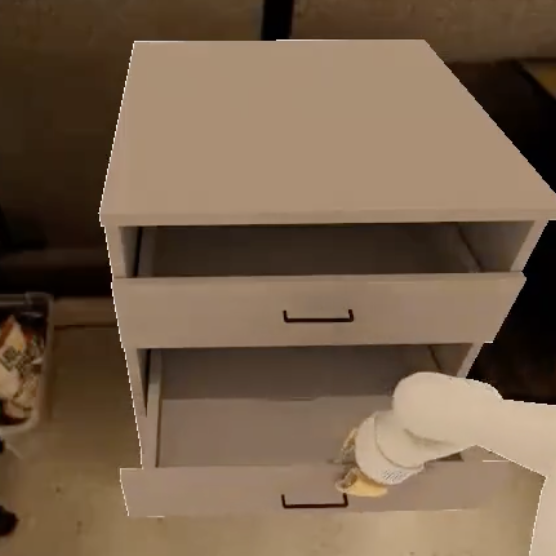
\includegraphics[width=\textwidth]{figures/examples/1.png}
          \end{minipage}%
          \begin{minipage}{0.33\linewidth}
            \centering
            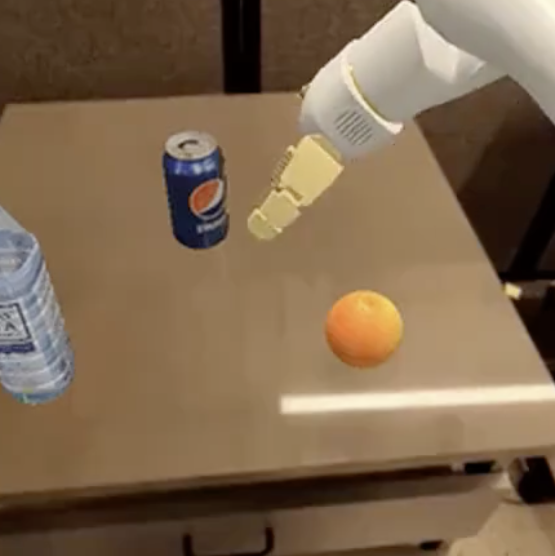
\includegraphics[width=\textwidth]{figures/examples/2.png}
          \end{minipage}%
          \begin{minipage}{0.33\linewidth}
            \centering
            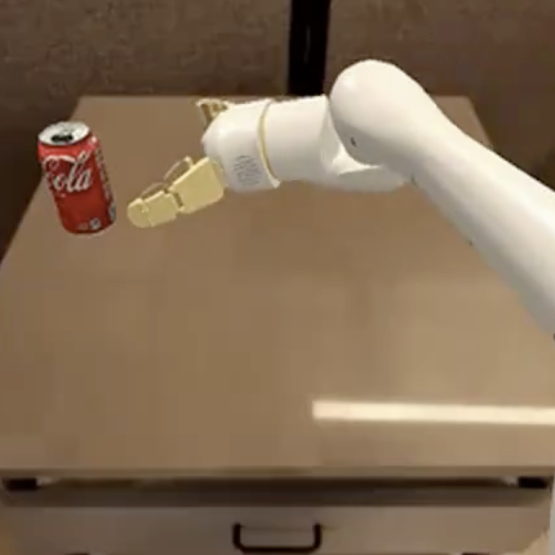
\includegraphics[width=\textwidth]{figures/examples/3.png}
          \end{minipage}
        \end{minipage}\vspace{-1.5ex}
        \begin{minipage}{\linewidth}
          \centering
          \begin{minipage}{0.33\linewidth}
            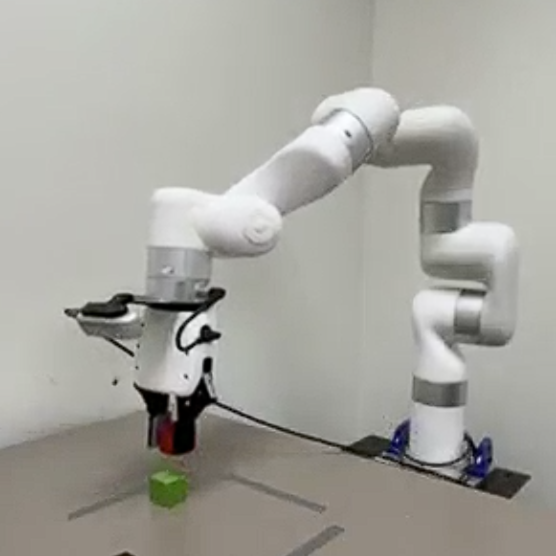
\includegraphics[width=\textwidth]{figures/examples/4.png}
          \end{minipage}%
          \begin{minipage}{0.33\linewidth}
              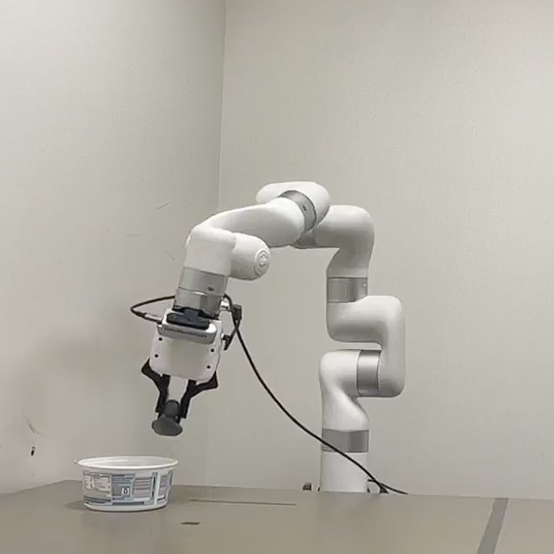
\includegraphics[width=\textwidth]{figures/examples/5.png}  
            \end{minipage}%
          \begin{minipage}{0.33\linewidth}
            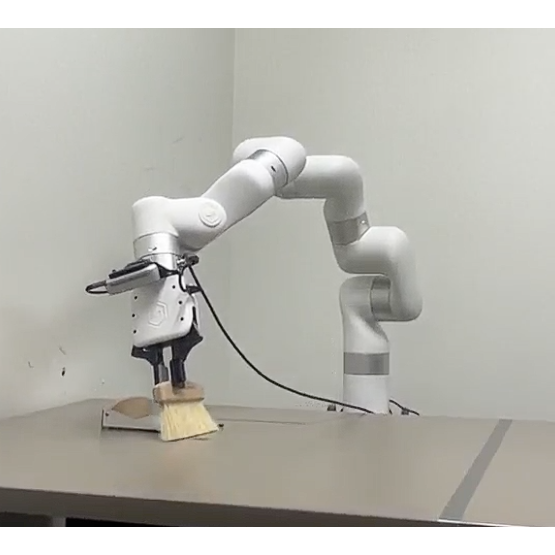
\includegraphics[width=\textwidth,trim={10pt 0 50pt 0},clip]{figures/examples/6.png}
          \end{minipage}\vspace{-2.5ex}
          \caption{\small \textbf{(Top)} Simulation tasks from Simpler~\cite{li24simpler}: {Close drawer}, {Move closer}, and {Pick Coke Can}. \textbf{(Bottom)} 
          Xarm7: {Stack Cubes}, {Duck in Bowl}, and {Sweep}.}
          \label{fig:xarm7}
        \end{minipage}
    \end{minipage}%
  \hfill
  \vspace{-0.5ex}
    \begin{minipage}{0.4\textwidth}
      \centering
      \begin{minipage}{0.45\linewidth}
        \centering
        \includegraphics[width=\textwidth]{figures/results/sim_res.pdf}
      \end{minipage}
      \hfill
      \begin{minipage}{0.49\linewidth}
        \centering
        \includegraphics[width=\textwidth]{figures/results/real_res.pdf}
      \end{minipage}
      \vspace{-2.5ex}
      \caption{\small Performance of models on simulated (left) and real (right) robotic tasks.}
      \label{fig:res}
    \end{minipage}\vspace{-1ex}
\end{wrapfigure}\vspace{-2.5ex}
\\
\noindent\textbf{\cib{5} ACT~\cite{zhao2023learningFB}:} ACT is a VLA model that uses ResNet~\cite{resnet} as the vision encoder and transformer-based
conditional variational autoencoder (CVAE)~\cite{sohn2015learning} that generates a sequence of actions. The original ACT 
was designed to process visual data and joint positions without additional language instructions. 
Similar to Octo~\cite{team2024octo}, ACT processes the images (multiple views if available, \eg original ACT uses 4 camera views) through a ResNet model, adds positional embeddings, and feeds them into a transformer-based CVAE-encoder (along with joint positions) to generate a sequence of actions (projected using MLP to chunks of absolute joint positions) through the CVAE-decoder.
\begin{comment}
For example, for Bimanual robots, the observation includes 4 RGB images (4 cameras), each at $480\times640$ resolution, and joint positions for two robot arms (7+7=14 positions in total).
The ResNet processes each image ($480\times640\times3$) and outputs feature maps of 4 images $\times$ $15\times20\times512$.
These feature maps are flattened ($1200\times512$), added to positional embeddings, and fed into the transformer encoder with additional joint position information.
The transformer decoder processes the encoder output through cross-attention to generate a sequence of actions ($k \times 512$ where $k$ is the number of action chunks). To generate the final actions, the output is down-projected with an MLP to $k \times 14$ dimensions, corresponding to the target joint positions for the next $k$ steps.
\end{comment}
Our implementation of ACT follows the original design, but changes are adopted to accommodate other embodiments, \eg change the number of views and action dimensions.%, \eg the Xarm7 robot has 1 camera view (additional views can be added) and 7 action dimensions (7 degree-of-freedom positions).
\\
\BfPara{Preliminary Experiments: Robotic Models} 
We have conducted preliminary experiments to evaluate the performance of robotic models, \ie RT-1, RT-2, Octo, and ACT on simulated and real robotic tasks. 
For simulation, we used Simpler~\cite{li24simpler} benchmark for three tasks: \emph{Close the drawer}, \emph{Move closer}, and \emph{Pick the Coke Can} using Google robot embodiment, while for real experiments, we used Xarm7 robot for three tasks: \emph{Stack Cubes}, \emph{Duck in Bowl}, and \emph{Sweep} (see~\autoref{fig:xarm7}).
For the simulation tasks, models were fine-tuned (using single third-person view and language-conditioned control) using 50 episodes per task. Language instructions are not used for ACT. Five training runs were performed per model, where each run was trained for 20,000 iterations with a batch size of 512 and a learning rate of 1e-5 using AdamW optimizer. The evaluation was performed on 25 episodes per task over five runs with different random seeds.
Similar training and evaluation settings were used for the real robotic tasks, but with visual observations only and no language instructions to avoid any changes on the ACT model architecture. 
Task success is measured using a two-point scoring system. For \emph{Stack Cubes} (stacking two cubes) and \emph{Duck in a bowl} (placing duck in bowl), points are awarded for successful pick (1 point) and place (1 point) operations. For \emph{Sweep}, points are given for finding (1 point) and sweeping objects into the bin (1 point). The success rate is calculated as the average scores divided by the total points in all evaluation episodes.
The preliminary results are shown in~\autoref{fig:res}.

% \BfPara{Adoption and Constraints}
% At inference time, each model is required to run at the rate required for the robot (3-10~Hz). 
% While relatively small models, \eg ACT, Octo, RT-1 can run locally on some robots with such inference rate, larger models, \eg OpenVLA and RT-2 (7B+ parameters), are hosted on a cloud service and queried over the network. This can introduce latency and network reliability issues, which are critical for real-time robotic applications.
% Even when designing/training such models to generate chunks of actions at once, which can be executed over several time steps,
% robotic models require strict real-time performance for smooth operation. % unlike general LLM/VLMs which often operate without stringent timing constraints.
% This adds complexity to robotic models, \ie managing latency, network reliability, and data communication security aspects that are less critical in typical LLM/VLM applications.
% In terms of adversarial attacks, attacking a robot's availability through prompt injection or jailbreak attacks (\eg running prompts that take more than 15Hz) can have far more serious consequences than similar attacks on other LLM/VLM applications.
% Compromised availability (and/or functionality) of a robot from an attack can cause physical harm, property damage, or operational disruptions.
% The real-time and/or (network dependence) of these models adds vulnerabilities that can be exploited to disrupt availability, making it imperative to prioritize security and resilience against such attacks.




\subsection{T1: Vulnerability Analysis in Foundation Generalist Robots}

This task aims to secure emerging robotic foundation models, where security and robustness are crucial.
% Vulnerabilities in AI models have been the focus of many studies recently, showing how small adversarial manipulations to the model's input can significantly impact their performance.
% Adversarial machine learning has emerged as an active field of research that addresses various threats to AI systems.
Based on the NIST Trustworthy and Responsible AI report~\cite{NIST_AI_100_2e2023}, the taxonomy of the most studied and effective attacks includes \emph{evasion}, \emph{poisoning}, \emph{privacy}, and \emph{abuse} attacks. % for generative AI systems.
For end-to-end robotic models, this task addresses all categories of attacks (\autoref{table:attacks_models}).%, including evasion, poisoning, privacy, and abuse attacks.
% Given the high-dimensional and multimodal nature of the search space for attacks aginst robotic models, simply introducing random noise to inputs might fail to identify subtle vulnerabilities of the robotic model.
% Moreover, robotic models/policies are generally designed to be resilient against such noise~\cite{miki2022scirob}, making such adversarial attacks ineffective using straightforward methods.
\\
\begin{wraptable}{r}{0.4\textwidth}
\centering 
\vspace{-7.5ex}
\caption{{\footnotesize Stages (Training and Inference), targets (Privacy, Integrity, Availability, and Abuse) and types ( White- (\dd), Gray- (\bb), and Black-box (\vv) ) of common Evasion, Poisoning, and Privacy attacks.}}\vspace{-2ex}
\label{table:attacks_models}
\small
\resizebox{0.98\linewidth}{!}{%
\begin{tblr}{
rowsep=0pt,
  column{3} = {c},
  column{4} = {c},
  column{5} = {c},
  column{6} = {c},
  column{7} = {c},
  column{8} = {c},
  column{9} = {c},
  cell{2}{1} = {r=8}{},
  cell{10}{1} = {r=10}{},
  cell{20}{1} = {r=6}{},
  hline{2,10,20,26} = {-}{},
}
                                                  &                                & \begin{sideways}Training\end{sideways} & \begin{sideways}Inference\end{sideways} & \begin{sideways}Privacy\end{sideways} & \begin{sideways}Integrity\end{sideways} & \begin{sideways}Availability\end{sideways} & \begin{sideways}Abuse\end{sideways} & \begin{sideways}Type\end{sideways} \\
\begin{sideways}Evasion      ~\end{sideways}      & Indirect Prompt Injection      & \ee                                       & \checkmark                                         & \checkmark                                       & \checkmark                                         & \checkmark                                            & \checkmark                                     & \vv                          \\
                                                  & Universal Adversarial Triggers & \ee                                       & \checkmark                                         & \ee                                      & \ee                                        & \ee                                           & \checkmark                                     & \vv                          \\
                                                  & Gradient-based Attacks         & \checkmark                                        & \checkmark                                         & \ee                                      & \ee                                        & \ee                                           & \ee                                    & \dd                          \\
                                                  & Prompt Injection               & \ee                                       & \checkmark                                         & \checkmark                                       & \checkmark                                         & \checkmark                                            & \checkmark                                     & \bb                           \\
                                                  & Refusal Suppression            & \ee                                       & \checkmark                                         & \ee                                      & \ee                                        & \ee                                           & \checkmark                                     & \bb                           \\
                                                  & Style Injection                & \ee                                       & \checkmark                                         & \ee                                      & \ee                                        & \ee                                           & \checkmark                                     & \bb                           \\
                                                  & Role-play Strategies           & \ee                                       & \checkmark                                         & \ee                                      & \ee                                        & \ee                                           & \checkmark                                     & \bb                           \\
                                                  & Jailbreak           & \ee                                       & \checkmark                                         & \ee                                      & \ee                                        & \ee                                           & \checkmark                                     & \bb                           \\
\begin{sideways}Poisoning         ~\end{sideways} & Data Poisoning                 & \checkmark                                        & \ee                                        & \ee                                      & \checkmark                                         & \checkmark                                            & \ee                                    & \dd                          \\
                                                  & Model Poisoning                & \checkmark                                        & \ee                                        & \ee                                      & \checkmark                                         & \checkmark                                            & \ee                                    & \dd                          \\
                                                  & Backdoor Poisoning             & \checkmark                                        & \checkmark                                 & \checkmark                                 & \checkmark                                        & \ee                                           & \checkmark                                     & \dd                          \\
                                                  & Label Flipping                 & \checkmark                                        & \ee                                        & \ee                                      & \checkmark                                         & \checkmark                                            & \ee                                    & \dd                          \\
                                                  & Clean-label Poisoning          & \checkmark                                        & \ee                                        & \ee                                      & \checkmark                                       & \ee                                           & \ee                                    & \dd                          \\
                                                  & Targeted Poisoning             & \checkmark                                        & \ee                                        & \ee                                      & \checkmark                                        & \ee                                           & \ee                                    & \dd                          \\
                                                  & Subpopulation Poisoning        & \checkmark                                        & \ee                                        & \ee                                      & \checkmark                                       & \ee                                           & \ee                                    & \dd                          \\
                                                  & Model Replacement              & \checkmark                                        & \ee                                        & \ee                                      & \checkmark                                        & \ee                                           & \ee                                    & \dd                          \\
                                                  & Model Boosting                 & \checkmark                                        & \ee                                        & \ee                                      & \checkmark                                        & \ee                                           & \ee                                    & \dd                          \\
                                                  & Functional Attacks             & \checkmark                                        & \ee                                        & \ee                                      & \checkmark                                        & \ee                                           & \ee                                    & \dd                          \\
\begin{sideways}Privacy\end{sideways}             & Data Reconstruction            & \ee                                       & \checkmark                                         & \checkmark                                       & \ee                                        & \ee                                           & \ee                                    & \vv                          \\
                                                  & Membership Inference           & \ee                                       & \checkmark                                         & \checkmark                                       & \ee                                        & \ee                                           & \ee                                    & \bb                           \\
                                                  & Model Extraction               & \ee                                       & \checkmark                                         & \checkmark                                       & \ee                                        & \ee                                           & \ee                                    & \vv                          \\
                                                  & Property Inference             & \ee                                       & \checkmark                                         & \checkmark                                       & \ee                                        & \ee                                           & \ee                                    & \bb                           \\
                                                  & Attribute Inference            & \ee                                       & \checkmark                                         & \checkmark                                       & \ee                                        & \ee                                           & \ee                                    & \bb                           \\
                                                  & Prompt and Context Stealing    & \ee                                       & \checkmark                                         & \checkmark                                       & \ee                                        & \ee                                           & \ee                                    & \vv                          
\end{tblr}
}{\vspace{3ex}}
\end{wraptable}\vspace{-5ex}
\\
\BfPara{Challenges} 
Attacking robotic models
presents unique challenges due to their complex architectures, the multimodal nature of their input, restrictions on the output/action space, and the evolving landscape of security measures. 
% Understanding these challenges is crucial for developing effective attack strategies that help
% uncover vulnerabilities and improve the robustness of these models. 
Main challenges include the following:
{\cib{1}} \emph{{Multimodal Complexity}:} Generalist robotic models process/integrate data from multiple modalities, such as sensory/positions data, images, and text, to predict action sequences. %We believe that the efforts to build robotic foundation models will continue to grow and other modalities will be incorporated.
    % Creating effective attacks requires understanding and manipulating the intricate relationships and interactions among these modalities \cite{radford2021learning}. 
    % Consequently, 
    Creating adversarial examples that can deceive both the visual and language components is more challenging than focusing on one. %, such as attacks on vision models~\cite{abdukhamidov2023hardening,abdukhamidov2024singleadv} and LLM~\cite{chowdhury2024breaking}, or unimodal attacks VLM \cite{fan2024unbridled}.
{\cib{2}} \emph{{Model Scale and Complexity:}} Current robotic models involve large architectures containing millions to billions of parameters, making them highly complex and computationally expensive to attack.
    Examining adversarial attacks on such large models necessitates significant computational resources. % and sophisticated optimization methods.
{\cib{3}} \emph{{Attack Practicality and Transferability:}} 
    Adversarial scenarios against robotics should be practical, \ie scenarios in which robots are likely to face operational tasks. 
Therefore, attacks must be systematic and guided by practical experience in field robotics to ensure the plausibility and reflection of real-world scenarios. 
    Moreover, attack methods against similar LLMs/VLMs use white-, gray-, and black-box settings relying on prior knowledge of (exact or similar) models, training data, restrictions/constraints of the system or training a surrogate models. However, robotic applications and commercial vendors often do not share model details \cite{cheng2018query}. In practice, attackers can only query the model and observe the behavior of the robot/output of the model. Developing attacks that exploit multiple vulnerabilities \cite{biggio2018wild} or adapt to various threat vectors is necessary and requires various strategies.
    % Moreover, an effective attack should be undetectable/imperceptible by human/robot observer, which requires preserving the semantic traits of the benign sample. 
    % This requires well-designed constraints to restrict the type and size of the perturbation. 
    Numerous studies have shown that some attacks exhibit high transferability, \ie attacks on a given model can succeed on other similar models. This phenomenon derived the transfer-based black-box attacks.
    Nevertheless, attacks designed for similar LLMs/VLMs models might not always work effectively on other models, even if they share similar architectures. 
    Ensuring adversarial examples are transferable \cite{liu2016delving} across models and tasks requires understanding model-specific vulnerabilities and generalizable attack methods.





        % Highly improbable conditions, like disturbances significantly beyond normal environmental challenges, do not contribute effectively to our understanding of a controller's nuanced vulnerabilities. 
    
    %\item  \textbf{Interpretable and Explainable Attacks}: For attacks to be truly effective, attackers need to understand the internal workings and decision-making processes \cite{doshi2017towards} of VLMs. However, the black-box nature of many VLMs, coupled with their complexity, makes it difficult to interpret how and why an attack succeeds or fails.
    % \item  \textbf{Robustness to Defenses}: Many VLMs incorporate dynamic defense mechanisms that can adapt to detected adversarial activities. These defenses may include real-time monitoring, anomaly detection, and adaptive retraining. Therefore, attack strategies need to continuously evolve to stay ahead of these adaptive defenses, which require substantial computational resources and sophisticated algorithms.






\BfPara{Definitions: Attacking Robotic Foundation Models}
{Let $\mathcal{F}$ represent a robotic foundation model, which takes a tuple of inputs, \eg $(\{\bm{x}\}, \{\bm{t}\}, \{\bm{s}\}, \dots)$ representing input modalities (\ie a set (at least one) of images \{$\bm{x}\} \in \mathcal{X}$, set of text instructions $\{\bm{t}\} \in \mathcal{T}$, set of sensory/position data $\{\bm{s}\}\in \mathcal{S}$, and other available information) and outputs a set of tokenized actions $\mathcal{F}(\{\bm{x}\}, \{\bm{t}\}, \{\bm{s}\}, \dots)=\{\bm{a}_{out}\}$.
Since robots could have multiple embodiments/tasks (and various action spaces), some inputs could become a placeholder/masked $\oslash$ or nonexistent input to fit the model.}
%%{\vspace{-2ex}}
% Let $\mathcal{F}$ represent a robotic foundation model, which takes a tuple of inputs, \eg $(\{\bm{x}\}, \{\bm{t}\}, \{\bm{s}\}, \dots)$ representing input modalities (\ie a set (at least one) of images \{$\bm{x}\} \in \mathcal{X}$, set of text instructions \{$\bm{t}\} \in \mathcal{T}$, set of sensory/position data $\{\bm{s}\}\in \mathcal{S}$, and other available information) and outputs a set of tokenized actions $\mathcal{F}(\{\bm{x}\}, \{\bm{t}\}, \{\bm{s}\}, \dots)=\{\bm{a}_{out}\}$.
% Since robots could have multiple embodiments/tasks (and various action spaces), some inputs could become a placeholder/masked $\oslash$ or nonexistent modified to fit the model.
For example, RT-2 and OpenVLA models receive only images and textual instruction $\mathcal{F}(\{\bm{x}\}, \{\bm{t}\})=\{\bm{a}_{out}\}$, 
%RoboCat and RT-1 receive images and no text, $\mathcal{F}(\{\bm{x}\}, \oslash)=\bm{a}_{out}$, 
Octo receives images, text, and sensory data $\mathcal{F}(\{\bm{x}\}, \{\bm{t}\}, \{\bm{s}\})=\bm{a}_{out}$, and ACT receives only images and sensory data $\mathcal{F}(\{\bm{x}\}, \{\bm{s}\})=\{\bm{a}_{out}\}$.
If Octo is used for robots/datasets that do not provide text instructions, the model processes available inputs and masks unavailable ones $\mathcal{F}(\{\bm{x}\}, \oslash,\{\bm{s}\})=\{\bm{a}_{out}\}$.
The output $\{\bm{a}_{out}\}$ is one or chunks of actions, each is a sequence of tokens representing predicted actions.



The attack operation $\mathcal{M}(.)$ is defined as a perturbation function that alters the inputs (one or more 
modalities) to mislead the model into producing an incorrect/unintended output action.
% We denote attacks on robotic models as $\mathcal{M} (.)$, which can be applied to one or more input modalities, \eg images, text, and sensory data.
For example, $\mathcal{M}(\bm{x})$ attacks image inputs $\bm{x}$, $\mathcal{M}(\bm{t})$ attacks text inputs $\bm{t}$, and $\mathcal{M}(\bm{x}, \bm{t})$ attacks both images and instructions.
\ul{\emph{Adversarial specificity}} can be either \textbf{targeted} or \textbf{untargeted} against security concepts. % \emph{Integrity}, \emph{Confidentiality}, and \emph{Availability}.
% For simplicity, we denote attack specificity as $\mathcal{M}(.) \xrightarrow{{}_{\textbf{T}}}  \bm{a}_{out}'$ for targeted and $\mathcal{M}(.) \xrightarrow{{}_{\textbf{U}}}  \bm{a}_{out}'$ for untargeted attacks.
The \ul{\emph{attacks goals}} can be categorized into \textbf{evasion}, \textbf{poisoning}, and \textbf{privacy}, and can be \ul{launched either in \textbf{training} or \textbf{inference} phases}.
For example, $\mathcal{M}(\bm{x},\bm{t}) \xrightarrow{{}_{\textbf{U}}} \bm{a}_{out}'$ such that $\bm{a}_{out}' \neq \bm{a}_{out}$ is an untargeted evasion attack that alters the input pair $(\bm{x},\bm{t})$ to cause the model to produce an incorrect output $\bm{a}_{out}'$.
Similarly, $\mathcal{M}(\bm{t}) \xrightarrow{{}_{\textbf{T}}} \bm{a}_{jailbreak}$ is a targeted jailbreak attack that alters the input instructions to cause the model to produce a specific (undesired) output.
If the attack is designed such that $\mathcal{M}(\bm{x},\bm{t}) \xrightarrow{{}_{\textbf{U}}} \bm{a}_{out}'$ where $\bm{a}_{out}'$ reveals confidential information, this constitutes a privacy attack.
Depending on the level of the \ul{\emph{adversary's capabilities and knowledge}} on the victim model/data/system, adversarial attacks can be categorized into \textbf{white-box}, \textbf{gray-box}, and \textbf{black-box} attacks. 
% \autoref{table:attacks_models} shows the general adversarial attack on robotic models.
Several threat models can be defined based on the adversarial specificity/goals, timing of the attack (\eg training or inference), the extent of adversarial capabilities, and the knowledge about the target model/system (\eg model parameters, source code, and/or training data).
% \ul{This task explores many threat models spanning different categorizations as shown in}{~\autoref{table:attacks_models}}.
% \BfPara{Related Work}
% Concurrent efforts study adversarial and backdoor threats to VLA models, but each targets an isolated model or component. BadVLA~\cite{badvla} inserts backdoors into a single VLA through objective-decoupled optimization. AdvVLA~\cite{advvla} crafts adversarial perturbations against one VLA policy. AttackVLA~\cite{li2025attackvla} benchmarks attacks but fixes the model family and reports no defenses grounded in robot kinematics. DRIFT~\cite{tae2026drift} derails the denoising trajectory of a single flow-matching VLA with an adversarial patch. Our proposal differs on three axes. First, we impose kinematic and Jacobian constraints so attacks and defenses respect the robot's reachable action space rather than pixel-space budgets alone. Second, we measure physical-consequence outcomes across six robot embodiments rather than one platform. Third, we release a unified benchmark, VLA-SecBench, pairing a cross-model transferability matrix with a single multi-task detector (TACD), so attacks, defenses, and interpretability are evaluated under one protocol instead of per-paper settings.
\begin{wrapfigure}{r}{0.25\textwidth}
\vspace{-2ex}
\centering
% \hspace{-2ex}
\begin{minipage}{0.25\textwidth}
\begin{minipage}{\textwidth}
\centering
\includegraphics[width=0.81\textwidth]{figures/results/visual_white_box.pdf}\vspace{-2ex}
\caption{\footnotesize Success rate of white-box attacks on robotic models using visual perturbations.}
\label{fig:visual_white_box}
\end{minipage}
% \hspace{-4ex}
\begin{minipage}{\textwidth}
  \centering
  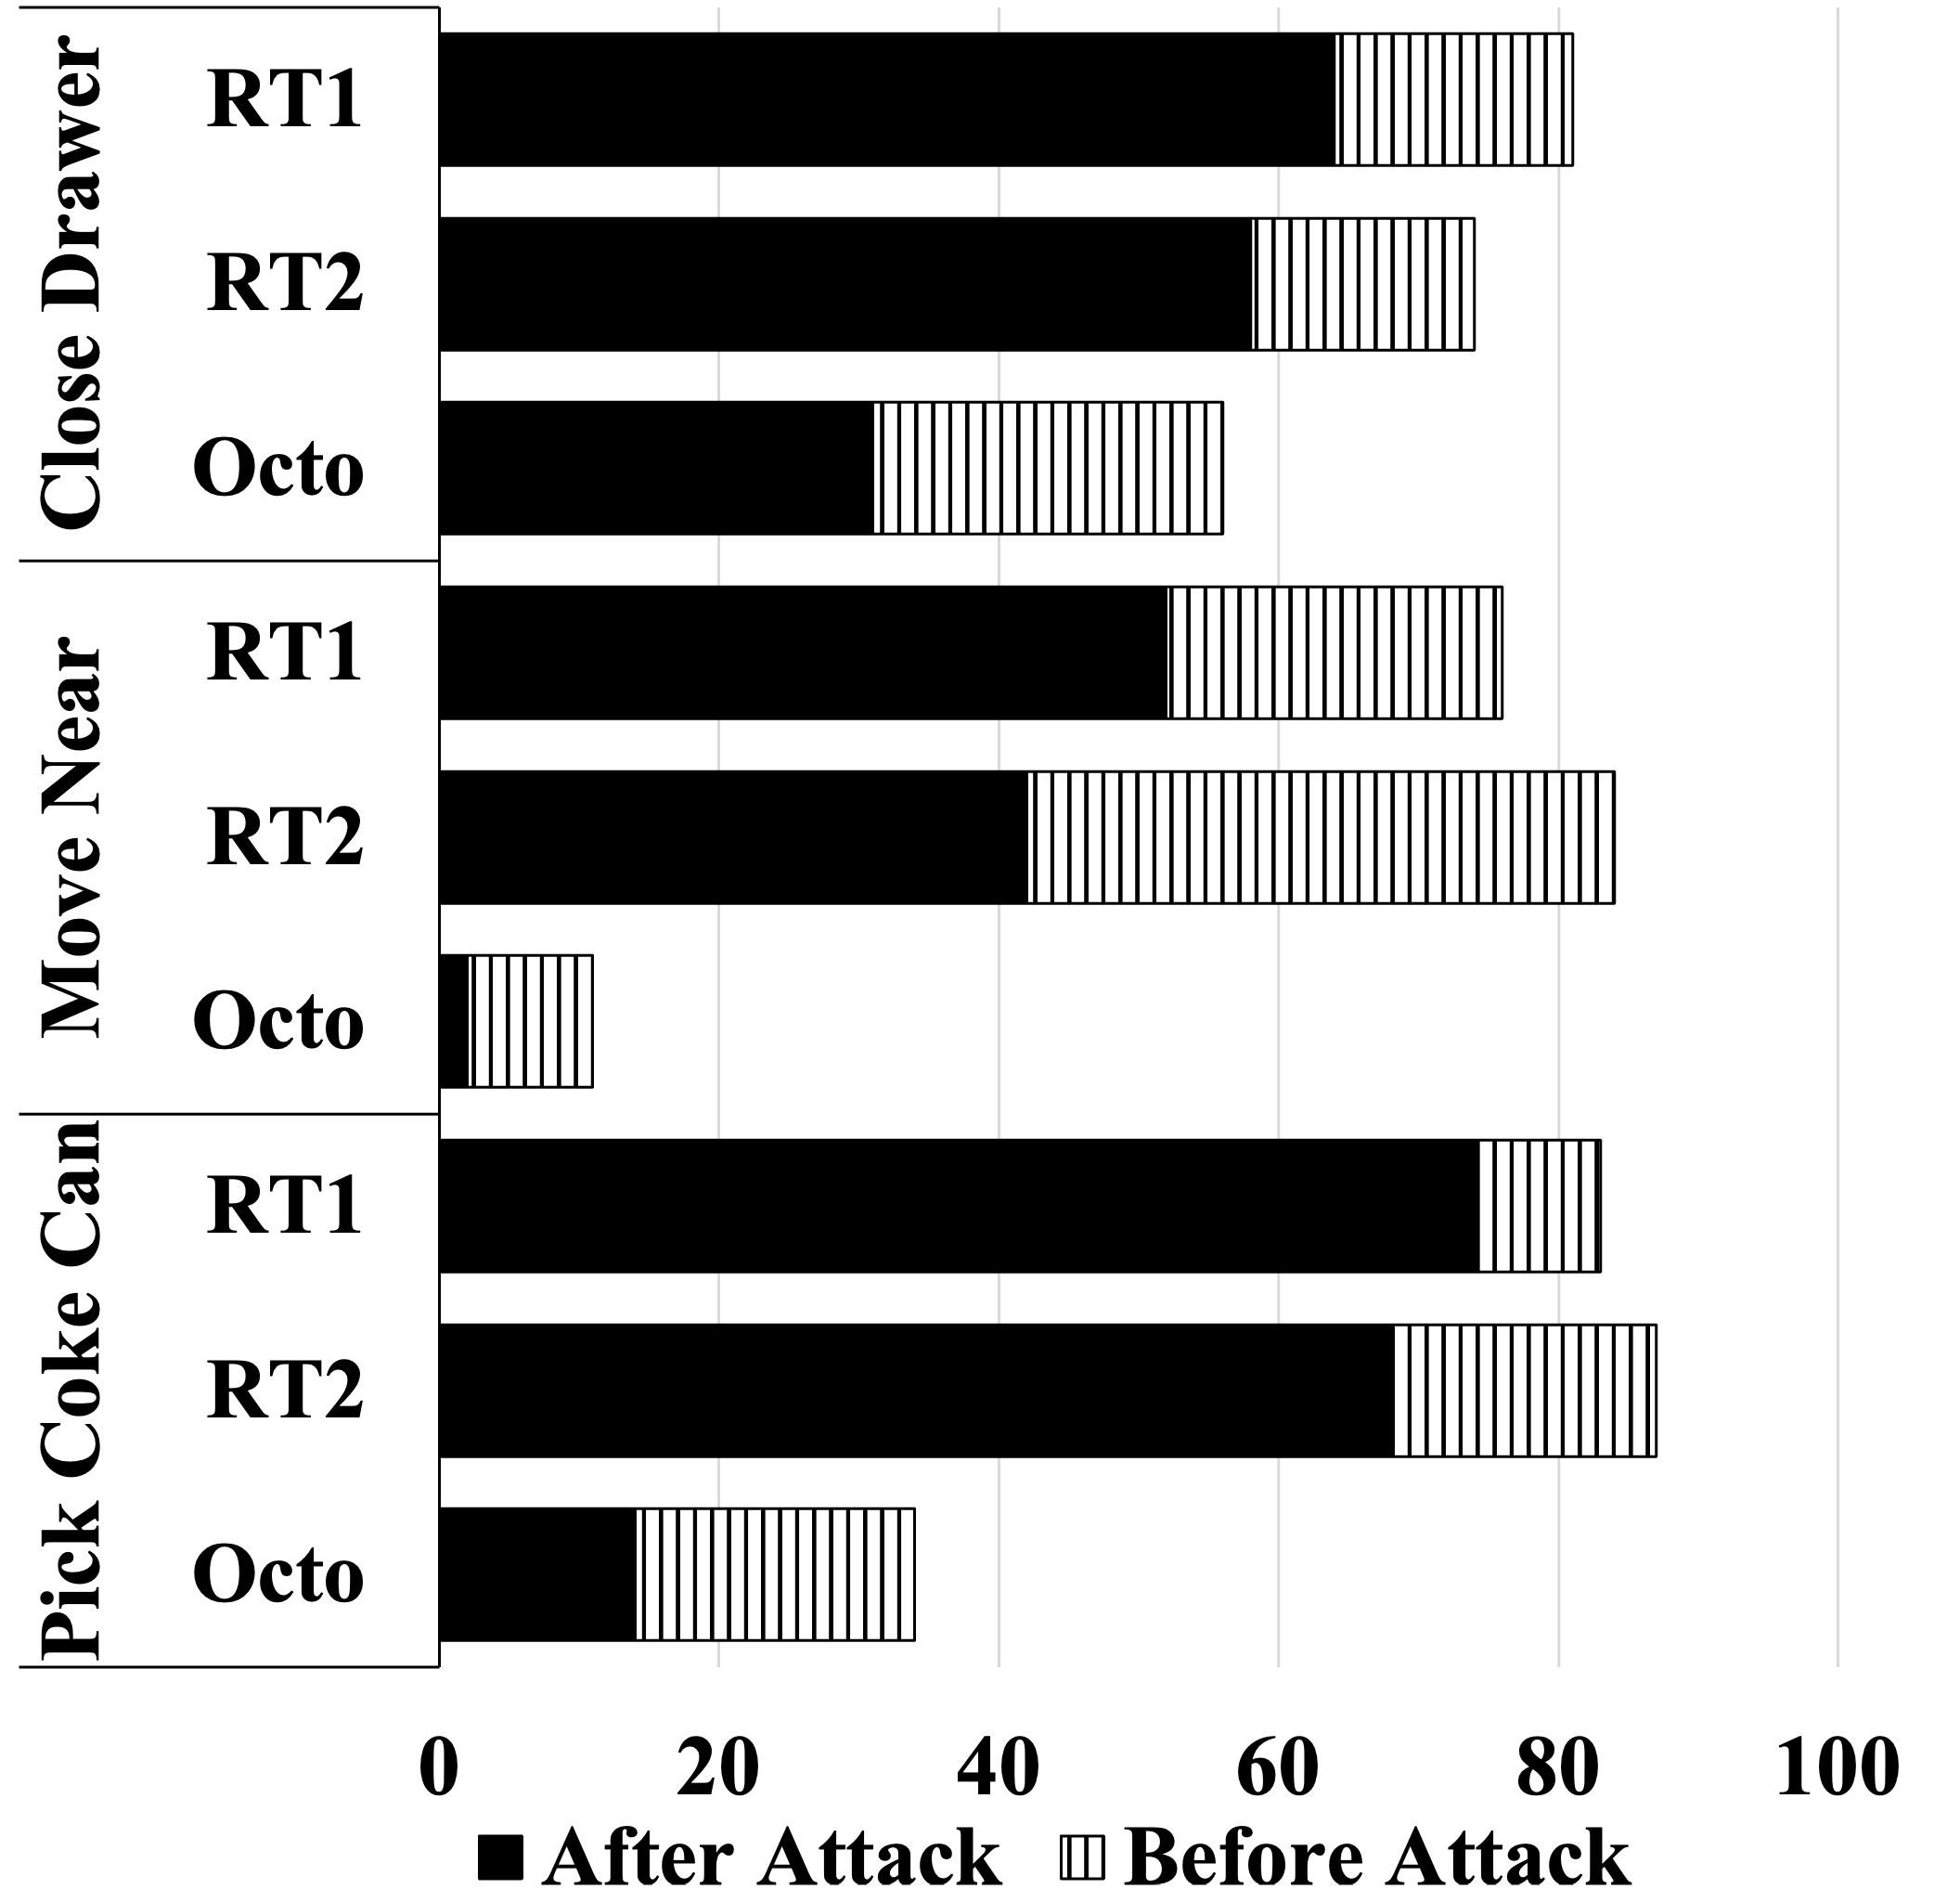
\includegraphics[width=0.74\textwidth]{figures/results/lang_black_box.pdf}\vspace{-2ex}
\caption{\footnotesize Task success rate of models before and after black-box token-based perturbations.}
  \label{fig:lang_black_box}
\end{minipage}
\end{minipage}
\vspace{-3ex}
\end{wrapfigure} 
\BfPara{Attacking Robotic Foundation Models: Preliminary Study}
We have conducted two preliminary experiments
 to evaluate the effectiveness of adversarial attacks on models trained on Simpler~\cite{li24simpler} benchmark using three tasks. Both experiments were conducted on the same three tasks as in the preliminary experiments, and evaluated using 25 episodes repeated 5 times.
\textbf{Experiment 1:} We examined \emph{untargeted white-box} attacks using visual perturbations (\ie on image inputs) against robotic models. We implemented three baseline attack methods: PGD~\cite{madry2017towards}, FGSM~\cite{goodfellow2014explaining}, and CW~\cite{carlini2017towards}. This attack scenario assumes the attacker has complete access to the parameters of the model's visual encoder, \ie EfficientNet-B3 (RT-1), Vision Transformer (RT-2), and ResNet (Octo and ACT). Such an assumption is realistic since these robotic models typically incorporate open-source pre-trained visual encoders. %, making their architecture and parameters readily available to potential attackers.
We evaluated the success rate of the attacks by measuring the percentage of successful adversarial examples where the generated actions differ from the ground-truth actions with a threshold of 30\%. \autoref{fig:visual_white_box} shows the attack success rate on various models. % using 25 episodes repeated 5 times.

\textbf{Experiment 2:} We examined \emph{black-box} attacks using token-based language perturbations (\ie on text inputs) against robotic models (except ACT as it does not support language instructions). We assume the attacker has no access to the model parameters and can only query the model. The attacker can manipulate the language instructions by deleting/replacing/adding tokens to the original instructions.
We adopted a similar attack approach to one used in SHIELD~\cite{abuhamad2025shield}, our previous work. %which focused on enhancing the robustness of code attribution models.
The attack perturbs 30\% of the tokens in the instructions with random tokens from the tokenizer vocabulary, and probes the model with a query limit of 500 queries. The attack terminates if the query limit is reached or if the model's output action differs from the ground-truth action by more than 30\%, in which case the attack is successful.
The results are shown
% {\vspace{-2.5ex}}
 in~\autoref{fig:lang_black_box}. %, where we observe that the success rate of the models drops significantly after the attack, indicating that even simple token-based perturbations can disrupt the model's performance.
These results demonstrate the potential vulnerabilities of robotic models to adversarial attacks.
% In these preliminary experiments we operationalized attack success as a 30\% action-token deviation. 
% In the full evaluation protocol described below, we use task success rate (TSR) under attack as the primary metric and use action deviation as a secondary physical-consequence metric.























\subsubsection{T1-1: White-box Attacks} \label{sec:t1_1}

White-box attacks exploit full access to the model's architecture and parameters.
White-box attacks provide deep insights into model vulnerabilities, enabling better understanding of its robustness.% and security of models, ensuring reliable and safe performance in real-world applications.
\\
\BfPara{Related Work} While the literature is rich in methods for white-box attacks against various models, the closest model families to generalist robot foundation models are VLMs.
Most evasion attacks against VLM \cite{schlarmann2023adversarial, bailey2023image,gao2024adversarial,wang2024stop,tan2024wolf} typically use gradient-based approaches, \eg PGD and CW, to generate/optimize perturbation for adversarial samples.
Recent work has begun to move beyond static, single-frame formulations toward trajectory-level redirection and architecture-specific attacks designed to flow-matching robot policies~\cite{puthumanaillam2026trajectory,tae2026drift}.
% As shown in \autoref{table:attacks_models}, gradient-based attacks can be performed in both the training and inference stages. During training, such attacks manipulate the model's learning process, leading to vulnerabilities such as various poisoning attacks, including recent objective-decoupled backdoor formulations against  VLA~\cite{zhou2025badvla}. At the inference stage, they generate adversarial examples by exploiting the model's gradients to deceive the model into making incorrect predictions. 
A recent study \cite{fu2023misusing} shows that seemingly harmless images with trojan-like characteristics can manipulate VLMs to call attacker-specific third-party tools or external APIs. 
% In a different study~\cite{cui2023robustness}, manipulating visual contents that are different from the VLM-specific domain is less effective in deceiving the model. 
Gao \etal \cite{gao2024inducing} introduce verbose images, creating imperceptible perturbations to make VLMs generate longer output sentences. Such an attack raises energy consumption and latency, which can have serious consequences in robotics.
% In a cross-modal analysis, creating and refining visual perturbations using adaptive prompts can identify numerous prompts that are effective with specific visual perturbations, resulting in high transferability of adversarial samples \cite{luo2024image}.
% Wu \etal \cite{wu2024adversarial} leverage adversarial text sequences to direct gradient-based perturbations on a single trigger image for attacking VLMs.
\ul{In this task, we propose new attack family, Action-Bin Boundary Perturbation (ABBP), and investigate the cross-modal behavior in evasion and poisoning scenarios against robotics models.}


% \newpage
\BfPara{Proposed Attack} 
We propose ABBP, a gradient-based white-box attack designed to exploit the uniform 256-bin discretization of the VLA action space. Because adjacent bins encode physically close but discretely different control signals, ABBP optimizes perturbations to drive predicted action tokens across bin boundaries.
Let $\mathcal{C}\subseteq\{1,\dots,d\}$ denote the $d$-dimensional continuous action, each uniformly quantized into $B{=}256$ bins, leaving $\{1,\dots,d\}\setminus\mathcal{C}$ for the discrete dimensions ({\eg} RT-1's arm/base/terminate mode). For $j\in\mathcal{C}$ the model $\mathcal{F}$ outputs logits $\bm{z}_j(\bm{\{x\}}, \bm{\{t\}})\in\mathbb{R}^{B}$, and the decoded bin and action are 
\vspace{-1ex}\begin{equation} 
  \small b_j=\argmax_{c\in\{0,\dots,B-1\}} z_{j,c}(\bm{\{x\}}, \bm{\{t\}}), \qquad \hat a_j=l_j+\bigl(b_j+\tfrac{1}{2}\bigr)\Delta_j, \qquad \Delta_j=\frac{u_j-l_j}{B}, 
  \label{eq:abbp-quant} 
\vspace{-1.5ex}
\end{equation} 
with $[l_j,u_j]$ the range of dimension $j$ and $\Delta_j$ the bin width. We set $\Delta_j{=}0$ for $j\notin\mathcal{C}$ and write $\hat{\bm{a}}\in\mathbb{R}^{d}$ and $\bm{\Delta}=[\Delta_1,\dots,\Delta_d]^{\top}$ for the decoded action and the bin-width vector. Uniform binning fixes $\Delta_j$ independently of the local sensitivity of the task, so a single-bin logit flip always carries a bounded but non-zero physical displacement. 
{\bf \emph{Kinematic map:}} Let $\mathcal{J}\subseteq\mathcal{C}$ index the dimensions driving the arm, excluding the gripper aperture and the base dimensions, so $|\mathcal{J}|{=}6$ in end-effector action spaces and $|\mathcal{J}|{=}n$ for an $n$-joint arm in joint space. For a joint configuration $\bm{\theta}$ and an action increment $\bm{u}\in\mathbb{R}^{d}$, the end-effector displacement over one control period $\tau$ is $G(\bm{\theta})\bm{u}\in\mathbb{R}^{6}$, where $G(\bm{\theta})\in\mathbb{R}^{6\times d}$ vanishes on columns outside $\mathcal{J}$ and restricts on $\mathcal{J}$ to $I_{6}$ for end-effector position spaces ({\eg} RT-1, RT-2, OpenVLA, and most of \autoref{tab:multi_dataset}), $\tau I_{6}$ for end-effector velocity spaces ({\eg} ConqHose, FMB), and the manipulator Jacobian $J(\bm{\theta})$ for joint-space actions ({\eg} ACT, RoboSet, SPOC), the last being the first-order approximation valid for the small increments considered here. These cover the action-space families of \autoref{tab:multi_dataset}. Because a twist mixes length and angle units, we measure displacement as $\|W G(\bm{\theta})\bm{u}\|_{2}$ with $W=\mathrm{diag}(1,1,1,\ell,\ell,\ell)$ and $\ell$ a characteristic lever arm of the embodiment.


% $G(\bm{\theta})$ enters the one-step target selection below. The gate metric instead measures the executed trajectory through forward kinematics, so it needs no linearization and applies unchanged to position and velocity action spaces.

ABBP exploits this structure in two stages.
\cib{1} \emph{Target selection:} ABBP selects a coordinated bin-shift vector $\bm{s}\in\mathbb{Z}^{d}$ maximizing end-effector displacement under budget and kinematic-feasibility constraints,
\vspace{-1ex}\begin{equation}
  \small
\bm{s}^{*}=\argmax_{\substack{\bm{s}\in\mathbb{Z}^{d},\; s_j=0\;\forall j\notin\mathcal{J}}}
\bigl\|W G(\bm{\theta})\,(\bm{s}\odot\bm{\Delta})\bigr\|_{2}
\;\;\text{s.t.}\;\;
\|\bm{s}\|_{1}\le\beta,\;\;
\|\bm{s}\|_{\infty}\le\sigma,\;\;
0\le b_j+s_j\le B-1,
\label{eq:abbp-shift}
\vspace{-1.5ex}\end{equation}
subject to $\hat{\bm{a}}+\bm{s}\odot\bm{\Delta}\in\mathcal{A}(\bm{\theta})$. Here $\odot$ is the
elementwise product, and $\beta$ and $\sigma$ are the total and per-dimension bin-shift budgets with
$\sigma<\beta$. The feasible set $\mathcal{A}(\bm{\theta})$ holds every action $\bm{a}$ obeying the
per-step velocity bound $\|\bm{a}-\hat{\bm{a}}\|_{\infty}\le\dot a_{\max}\tau$ for a per-dimension
action-rate limit $\dot a_{\max}$, and reaching a configuration $\psi(\bm{\theta},\bm{a})$ inside the
joint limits $\mathcal{L}$ and the reachable workspace $\mathcal{W}$ after one control period $\tau$.
The objective is convex in $\bm{s}$, so $\beta$ alone would spend the budget on the single
highest-gain dimension, while $\sigma$ spreads the shift across several degrees of freedom, and the
bin bounds keep $b_j+s_j^{*}$ decodable without post-hoc clipping.
\cib{2} \emph{Perturbation synthesis:} With $b_j^{*}=b_j+s_j^{*}$, ABBP solves a margin objective over the visual input (expandable to textual input as well),
\vspace{-3ex}\begin{equation}
  \small
\min_{\bm{\delta}}\;\sum_{j=1}^{d} w_j
\Bigl[\max_{c\neq b_j^{*}} z_{j,c}(\bm{x}+\bm{\delta},\bm{t})-z_{j,b_j^{*}}(\bm{x}+\bm{\delta},\bm{t})+\kappa\Bigr]_{+}
\quad\text{s.t.}\quad
\|\bm{\delta}\|_{\infty}\le\epsilon,\;\;\bm{x}+\bm{\delta}\in[0,1]^{N},
\label{eq:abbp-obj}
\vspace{-1.5ex}\end{equation}
where $\bm{\delta}$ is the additive image perturbation, $\epsilon$ its $\ell_{\infty}$ budget, and $N$ the number of pixel values in $\bm{x}$, with $[\cdot]_{+}=\max(\cdot,0)$, confidence margin $\kappa$, and box constraint in raw pixel space before encoder normalization. The weights are $w_j=\|(WG(\bm{\theta}))_{:,j}\|_{2}\Delta_j$ for $j\in\mathcal{J}$, so the optimizer allocates perturbation budget to the dimensions with the largest physical effect per bin, and $w_j=\lambda$ for $j\notin\mathcal{J}$. 
% Stage 1 fixes $s_j^{*}{=}0$ off $\mathcal{J}$, so $b_j^{*}{=}b_j$ there and the second group of terms pins the gripper aperture and the arm/base/terminate mode to their clean values. Without them $\bm{\delta}$ could flip the mode token to \emph{terminate}, which halts the episode and drives the displacement the attack optimizes for to zero. 
% For $j\notin\mathcal{C}$ the inner maximum runs over that dimension's own label set rather than the $B$ bins. 
\autoref{eq:abbp-obj} treats the $d$ logit vectors as conditionally independent, which holds for parallel readout heads ({\eg} RT-1, Octo). For autoregressive action decoders ({\eg} RT-2, OpenVLA), the action tokens form a sequence and $\bm{z}_j$ depends on the preceding tokens, so we evaluate each margin under teacher forcing on the target prefix $b^{*}_{<j}$. We solve \autoref{eq:abbp-obj} by projected gradient descent with step $\alpha$ over $T$ iterations. Setting $w_j{=}1$ for $j\in\mathcal{J}$ and $\sigma{=}1$ while retaining $\mathcal{A}(\bm{\theta})$ yields a discretization-agnostic variant, isolating the contribution of the physical-effect weighting in an ablation.


\BfPara{ABBP in Poisoning Scenarios} The two-stage design of ABBP extends from \emph{evasion} to training-time \emph{poisoning} attacks (see \autoref{table:attacks_models}). 
In evasion, ABBP perturbs the input under budget $\epsilon$. In poisoning, the attacker applies the
target selection $\bm{s}^{*}$ (\autoref{eq:abbp-shift}) and the margin objective
(\autoref{eq:abbp-obj}) to training data, action labels, or gradient updates, and we reinterpret the
attack budget as the poison rate, \ie the fraction of corrupted samples or updates.
For example,
because VLA action labels are bin indices, \emph{data poisoning} and \emph{label flipping} reduce to
setting $b_j \rightarrow b_j+s^{*}_{j}$ on the dimensions \autoref{eq:abbp-shift} selects, where a
shift of at most $\sigma$ bins encodes a physically adjacent action and evades label inspection. 
\emph{Backdoor poisoning} pairs a visual or textual trigger with labels fixed at $b_j^{*}=b_j+s_j^{*}$, so the trigger induces a kinematically feasible displacement of maximal magnitude at inference, while \emph{clean-label} and \emph{targeted} poisoning variants keep labels intact and instead
perturb the observation so the model binds a context to the shifted mapping $b^{*}_{j}$. 
\emph{Subpopulation poisoning} concentrates corrupted samples on configurations with high kinematic
gain $\|(WG(\bm{\theta}))_{:,j}\|_{2}$, limiting degradation on clean data outside the target
subpopulation.
\emph{Model poisoning}, \emph{model replacement}, and \emph{model boosting} assume gradient- or model-channel access, \eg federated fine-tuning or fine-tuning-as-a-service, and use the ABBP margin as an auxiliary training loss, biasing logits near bin boundaries while clean task success stays high. \emph{Functional attacks} follow the same pattern, poisoning the learned policy toward systematic violation of a behavioral property such as the per-step velocity bound $\|\bm{a}-\hat{\bm{a}}\|_{\infty}\le\dot a_{\max}\tau$. 
% We evaluate all poisoning variants under the physical-consequence metric of \autoref{eq:abbp-gate}, with the poison rate taking the role of the budget.
%%%%%%%%%%%%%%%%%%%%%%%%%%%%%%%%%%%%%%%



\BfPara{Attack Evaluation Protocol} All T1 attack families are evaluated under one protocol with
three metrics computed from a single episode. 
Let $\mathcal{E}$ be the evaluation episodes of a task ($|\mathcal{E}|{=}25$) and $\mathcal{I}$ the independent seeds ($|\mathcal{I}|{=}10$). Each
episode $e\in\mathcal{E}$ is run twice from an initial state, once on clean observations and once with $\mathcal{M}$ active at budget $\epsilon$, re-optimized at every step. 
For inference-time attacks, $\epsilon$ is the $\ell_{\infty}$ bound of \autoref{eq:abbp-obj}; for training-time attacks it is the poison rate. 
In both cases $\epsilon$ is drawn from a fixed geometric grid $E$ capped at $\epsilon_{\max}$. A run returns a task score $v_{\mathcal{M}}(e,\epsilon)\in[0,1]$ under the two-point scoring of \autoref{sec:t0}, the end-effector poses $(\bm{p}_{k},R_{k})$ and $(\bm{p}'_{k},R'_{k})$ for $k=0,\dots,H$ from forward kinematics, and the decoded bins $b_{j,k}$ and $b'_{j,k}$ of \autoref{eq:abbp-quant}.
We write $v_{0}(e)=v_{\mathcal{M}}(e,0)$ and $\mathcal{E}_{0}=\{e\in\mathcal{E}:v_{0}(e)=1\}$ for the episodes the undefended policy completes. We fix $H$ at one quarter of the median episode of the embodiment. We measure the following metrics.

\cib{1} \textbf{Physical consequence.} Comparing the two pose sequences,
\vspace{-1ex}\begin{equation}
  \small
\bm{e}_{k}=\begin{bmatrix}\bm{p}'_{k}-\bm{p}_{k}\\[2pt] rv\bigl(R_{k}^{\top}R'_{k}\bigr)\end{bmatrix},
\qquad
D^{e}_{\mathcal{M}}(H)=\bigl\|W\bm{e}_{H}\bigr\|_{2},
\qquad
\bar{D}^{e}_{\mathcal{M}}(H)=\max_{0\le k\le H}\bigl\|W\bm{e}_{k}\bigr\|_{2},
\label{eq:abbp-gate}
\vspace{-1.5ex}\end{equation}
where $rv$ is the rotation-vector map of the relative rotation and $W=\mathrm{diag}(1,1,1, \ell,\ell,\ell)$ weights rotational displacement by the characteristic lever arm $\ell$ of the embodiment, so that $D$ and $\bar{D}$ carry units of length. $D^{e}_{\mathcal{M}}(H)$ is the terminal deviation, written $D_{\mathcal{M}}(H)$ when the episode is implicit; the peak deviation $\bar{D}^{e}_{\mathcal{M}}(H)$ is also reported. The threshold $\rho$ is calibrated per task (\ie based on the gripper-aperture clearance and the size of manipulated object, \eg $\rho{=}5$\,cm in preliminary tasks).
\cib{2} \textbf{Task and attack success.} From the same runs,
\vspace{-1ex}\begin{equation}
  \small
\mathrm{TSR}_{\mathcal{M}}(\epsilon)=\frac{1}{|\mathcal{E}|}\sum_{e\in\mathcal{E}}
v_{\mathcal{M}}(e,\epsilon),
\quad
\mathrm{ASR}^{\mathrm{task}}_{\mathcal{M}}(\epsilon)=\frac{1}{|\mathcal{E}_{0}|}
\sum_{e\in\mathcal{E}_{0}}\mathbb{1}\bigl[v_{\mathcal{M}}(e,\epsilon)<1\bigr],
\quad
\mathrm{ASR}^{\mathrm{phys}}_{\mathcal{M}}(\epsilon)=\frac{1}{|\mathcal{E}|}
\sum_{e\in\mathcal{E}}\mathbb{1}\bigl[D^{e}_{\mathcal{M}}(H)\ge\rho\bigr],
\label{eq:metric-stack}
\vspace{-1.5ex}\end{equation}
and, at the token level,
$\mathrm{ASR}^{\mathrm{tok}}_{\mathcal{M}}(\epsilon)=(|\mathcal{E}|H)^{-1}\sum_{e,k}
\mathbb{1}[\exists j\in\mathcal{J}:b'_{j,k}\neq b_{j,k}]$ for untargeted attacks, replaced by
$\mathbb{1}[\exists j:b'_{j,k}{=}b^{*}_{j,k}]$ and $\mathbb{1}[b'_{j,k}{=}b^{*}_{j,k}\,\forall
j\in\mathcal{J}]$ for the targeted \textit{Contain} and \textit{Exactmatch} criteria
\cite{lu2024test,luo2024image}, with $b^{*}_{j}$ the target bin of \autoref{eq:abbp-shift}.
Conditioning $\mathrm{ASR}^{\mathrm{task}}$ on $\mathcal{E}_{0}$ prevents baseline policy
failures from inflating it. 
%A token flip is necessary but not sufficient for displacement,
% which is necessary but not sufficient for task failure, so we expect
% $\mathrm{ASR}^{\mathrm{task}}\le\mathrm{ASR}^{\mathrm{phys}}\le\mathrm{ASR}^{\mathrm{tok}}$. 
\cib{3} \textbf{Attack cost and comparison.} For an effect $\Phi$ and threshold
$\rho_{\Phi}$,
\vspace{-1ex}\begin{equation}
  \small
\epsilon^{*}_{\mathcal{M}}(\Phi,\rho_{\Phi})=\min\bigl\{\epsilon\in E:\;
\widehat{\mathbb{E}}\bigl[\Phi_{\mathcal{M}}(\epsilon)\bigr]\ge\rho_{\Phi}\bigr\},
\qquad
\hat{\gamma}^{\,i}_{\mathcal{M}_{b}}=
\frac{\epsilon^{*,i}_{\mathcal{M}_{b}}(\Phi,\rho_{\Phi})}
{\min_{\mathcal{M}\in\{\mathcal{M}_{1},\dots,\mathcal{M}_{m}\}}
\epsilon^{*,i}_{\mathcal{M}}(\Phi,\rho_{\Phi})},
\label{eq:budget-operator}
\vspace{-1.5ex}\end{equation}
with $\epsilon^{*}_{\mathcal{M}}=\epsilon_{\max}$ when no grid point reaches $\rho_{\Phi}$, the expectation taken over $\mathcal{E}$, and $\epsilon^{*,i}$ the value estimated on seed $i\in\mathcal{I}$. 
% We instantiate $\Phi$ three ways: the task instantiation $\epsilon^{*}_{\mathrm{TSR}}=\epsilon^{*}\bigl(1-\mathrm{TSR}_{\mathcal{M}}(\epsilon)/ \mathrm{TSR}_{\mathcal{M}}(0),\,\rho_{\mathrm{TSR}}\bigr)$ with $\rho_{\mathrm{TSR}}{=}0.5$, the budget that halves task success, which is our primary metric; the physical instantiation $\epsilon^{*}_{\mathrm{phys}}=\epsilon^{*}(D_{\mathcal{M}}(H),\rho)$, which resolves attacks whose displacement has not yet crossed a task boundary; and the token instantiation $\epsilon^{*}_{\mathrm{tok}}=\epsilon^{*}(\mathrm{ASR}^{\mathrm{tok}}_{\mathcal{M}},0.5)$, which requires forward passes only. 
We define $\Phi$ in three forms, based on the task success, the physical displacement, and the action-token-level attack success. For the task form, 
$\epsilon^{*}_{\mathrm{TSR}}=\epsilon^{*}(1-\mathrm{TSR}_{\mathcal{M}}(\epsilon)/
\mathrm{TSR}_{\mathcal{M}}(0),\,0.5)$ is the budget halving task success. 
The physical form $\epsilon^{*}_{\mathrm{phys}}=\epsilon^{*}(D_{\mathcal{M}}(H),
\rho)$ resolves displacement below task failure. The token form
$\epsilon^{*}_{\mathrm{tok}}=\epsilon^{*}(\mathrm{ASR}^{\mathrm{tok}}_{\mathcal{M}},
0.5)$ needs forward passes only.
We report $\mathcal{M}_{b}$ as a distinct vulnerability over $\mathcal{M}_{1},\dots,\mathcal{M}_{m}$ when the median of $\hat{\gamma}^{\,i}_{ \mathcal{M}_{b}}$ over $\mathcal{I}$ satisfies $\hat{\gamma}_{\mathcal{M}_{b}}\le\gamma$ on $\epsilon^{*}_{\mathrm{TSR}}$ for at least two of three tasks. Weaker adversarial knowledge relaxes $\gamma$ ($\gamma{=}0.7$ in white-box, $\gamma_{g}{=}0.8$ in gray-box, $\gamma_{b}{=}0.9$ in black-box).

\BfPara{Defense Evaluation Protocol}
Under the same protocol, for each attack $\mathcal{M}$,
\vspace{-1ex}\begin{equation}
  \small
\mathcal{C}_{\mathcal{M}}=\frac{\epsilon^{*}_{\mathcal{M}}(\Phi,\rho_{\Phi})\big|_{\mathrm{def}}}
{\epsilon^{*}_{\mathcal{M}}(\Phi,\rho_{\Phi})\big|_{\mathrm{undef}}},
\qquad
\mathcal{T}=\mathrm{TSR}^{\mathrm{def}}(0)-\mathrm{TSR}(0),
\qquad
\mathrm{TPR}_{\mathcal{M}}\ \text{at}\ \mathrm{FPR}\le0.01,
\label{eq:defense-metrics}
\vspace{-1.5ex}\end{equation}
where $\mathcal{C}_{\mathcal{M}}$ is the multiplicative attack-cost increase, $\mathcal{T}$ the clean-task
cost of the defense, and $\mathrm{TPR}_{\mathcal{M}}$ the TACD detection rate at the threshold
$\xi_{t}$ calibrated on held-out benign episodes. 
% TACD is effective when $\mathrm{TPR}_{\mathcal{M}}\ge0.9$ for ABBP, STAP, and TTDA on at least two of three tasks, including against an adaptive adversary that knows $\xi_{t}$ and the forecaster. AGAT is effective when $\mathcal{C}_{\mathcal{M}}\ge2$ for every attack with $\mathcal{T}\ge-0.05$, or when it degrades each attack to the level of the best baseline defense (input smoothing, VLM-ported adversarial training, ensemble voting).

% \emph{Estimation and statistics.} Episodes are clustered within seeds, so all quantities are aggregated to one value per seed and compared on the $|\mathcal{I}|$ paired per-seed values with a one-sided Wilcoxon signed-rank test at $p<0.05$, Holm-corrected across tasks. Uncertainty is reported as a cluster-bootstrap 95\% confidence interval resampling seeds and then episodes within seed, and as mean~$\pm$~std. Privacy attacks carry no task notion and fall outside \autoref{eq:metric-stack}: membership inference reports true-positive rate at a 1\% false-positive rate over the score $r(e)$ of \autoref{sec:t1_2}, and model extraction reports action-agreement fidelity. Full episode run is required only for $\mathrm{TSR}$ and $\mathrm{ASR}^{\mathrm{phys}}$, so we populate the full model~$\times$~model~$\times$~attack transferability matrix with $\mathrm{ASR}^{\mathrm{tok}}$, run full episodes on a stratified calibration subset, and report Kendall's $\tau_{b}$ between $\mathrm{ASR}^{\mathrm{tok}}$ and $\epsilon^{*}_{\mathrm{TSR}}$ to establish whether the token-level screen is a valid proxy.
%%%%%%%%%%%%%%%%%%%%%%%%%%%%%%%%%%%%%%

% \BfPara{Evaluation Protocol} All T1 attack families are evaluated under one physical-consequence protocol. A single bin crossing displaces the end-effector by a fraction of a millimeter, which no task-level metric resolves, so we measure consequence as the cumulative deviation of a run. From an initial state, we run the policy for $H$ steps twice, once on clean observations and once with the attack re-optimized at every step, and compare the two end-effector poses $(\bm{p}_k,R_k)$ and $(\bm{p}'_k,R'_k)$ at each step $k=0,\dots,H$ obtained by forward kinematics,
% \vspace{-1ex}\begin{equation}
%   \small
% \bm{e}_{k}=\begin{bmatrix}\bm{p}'_{k}-\bm{p}_{k}\\[2pt]{rv}\bigl(R_{k}^{\top}R'_{k}\bigr)\end{bmatrix},
% \qquad
% D_{\mathcal{M}}(H)=\bigl\|W\bm{e}_{H}\bigr\|_{2},
% \qquad
% \epsilon^{*}_{\mathcal{M}}(\rho)=\min\Bigl\{\epsilon\in E:\;
% \widehat{\mathbb{E}}\bigl[D_{\mathcal{M}}(H)\bigr]\ge\rho\Bigr\},
% \label{eq:abbp-gate}
% \vspace{-1.5ex}\end{equation}
% where $\mathcal{M}$ ranges over the attacks under comparison, ${rv}$ is the rotation-vector map of the relative rotation, 
% $D_{\mathcal{M}}(H)$ is the consequence at the final step $H$ with displacement of $\bm{e}_{H}$ weighted by $W$, 
% $E$ is a fixed geometric grid of budgets capped at $\epsilon_{\max}$, $\epsilon^{*}_{\mathcal{M}}(\rho)=\epsilon_{\max}$ when no grid point reaches $\rho$, and the expectation runs over evaluation episodes. 
% % where $W=\mathrm{diag}(1,1,1,\ell,\ell,\ell)$ weights rotational displacement by the characteristic lever arm $\ell$, $E$ is a fixed geometric grid of budgets capped at $\epsilon_{\max}$, and the expectation runs over evaluation episodes. 
% We fix $H$ steps at one quarter of the median robot episode, and estimate $\epsilon^{*}$ independently for each of ten seeds. We report an attack as a distinct vulnerability at (\eg $\rho{=}5$\,cm the cumulative deviation threshold in our experiments) when its $\epsilon^{*}(\rho)$ improves over the best baseline by a threat-tier factor on at least two of three tasks, under a one-sided Wilcoxon signed-rank test at $p<0.05$ on the paired per-seed ratios.
% The $\epsilon^{*}_{\mathcal{M}}(\rho)$ defines the smallest budget $\epsilon$ on grid $E$ at which attack $\mathcal{M}$ achieves a consequence meeting or exceeding $\rho$.
% So, an attack $\mathcal{M}_b$ is distinct over attacks (\eg $\mathcal{M}_1,\dots,\mathcal{M}_m$) if $\epsilon^{*}_{{\mathcal{M}_b}}(\rho)\le\gamma\,\min_{\mathcal{M}\in\{\mathcal{M}_1,\dots,\mathcal{M}_m\}}\epsilon^{*}_{\mathcal{M}}(\rho)$.
% Weaker adversarial knowledge relaxes $\gamma$ ($\gamma{=}0.7$, $0.8$, $0.9$ for white-, gray-\autoref{sec:t1_2}, and black-box \autoref{sec:t1_3}, respectively). Training-time attacks use the poison rate as budget. Metrics are reported as mean~$\pm$~std across runs. 

\BfPara{ABBP Evaluation} We evaluate ABBP under the shared protocol (\autoref{eq:abbp-gate}) with $\gamma{=}0.7$ and baselines PGD, FGSM, and CW. We calibrate $(\sigma,\rho)$ against the reachability bound $\rho\le H\sqrt{|\mathcal{J}|}\,\sigma\max_{j\in\mathcal{J}}\|(WG(\bm{\theta}))_{:,j}\|_{2}\Delta_{j}$ implied by \autoref{eq:abbp-quant} and \autoref{eq:abbp-shift}, so the target remains reachable before any experiment runs. We also report the discretization-agnostic ablation ($w_j{=}1$, $\sigma{=}1$) to isolate the contribution of the physical-effect weighting.


\subsubsection{T1-2: Gray-box Attacks} \label{sec:t1_2}
Gray-box attacks exploit partial knowledge of the victim model, \eg the architecture and training data, to expose vulnerabilities under moderate adversarial capabilities. For example, existing gray-box attacks against VLMs use open-source vision or language encoders as surrogates to launch the attack.
Attacks include \emph{prompt injection} and \emph{jailbreak} for evasion and \emph{membership}, \emph{property}, and \emph{attribute inference} for privacy (\autoref{table:attacks_models}).

\BfPara{Related Work} Zhao \etal~\cite{zhao2024evaluating} align adversarial perturbations with CLIP~\cite{radford2021learning} and BLIP~\cite{li2022blip} embeddings to generate transferable adversarial examples. Wang \etal~\cite{wang2024transferable} disrupt modality-consistency features in critical attention regions. Wu \etal~\cite{wu2024adversarial} embed adversarial sub-images within larger images to attack GPT-4o, Gemini, and Claude. Prior work measures transfer success on the text or image outputs of VLMs, not on the actions of a robot policy, and relies on fixed public surrogates with no control over the surrogate training.
\ul{In this sub-task, we propose a new attack family, Surrogate-Transfer Action Perturbation (STAP), and we study gray-box privacy attacks against robotic models.}

\BfPara{Proposed Attack} We propose STAP, a surrogate-transfer gray-box attack grounded in the action space of the robot. Let a victim policy  $\mathcal{F}=(\mathcal{P},\bm{\omega})$, where $\mathcal{P}$ collects the public components (\eg the vision encoder, the VLM backbone, and the action tokenizer) and $\bm{\omega}$ collects the private components (\eg fine-tuned policy weights, the action head, and the data mixture). The gray-box adversary knows $\mathcal{P}$ and the architecture family but not $\bm{\omega}$. 
This assumption matches deployments of Octo and OpenVLA, whose base components are public while embodiment-specific checkpoints and training data remain private. For victims on closed backbones (\eg RT-2 with PaLI-X), the adversary substitutes the closest public VLM (see \autoref{tab:VLMs}). %Component knowledge separates this setting from the black-box setting of \autoref{sec:t1_3}, where the adversary knows no component and builds a generic surrogate.

The attacker constructs a surrogate policy $\mathcal{F}'$ by fine-tuning the same components $\mathcal{P}$ on the public data mixture of \autoref{tab:multi_dataset} with independent splits and seeds, so $\mathcal{F}'$ matches $\mathcal{F}$ in architecture, tokenizer, and task distribution but not in weights or demonstrations. 
STAP realizes an untargeted evasion attack $\mathcal{M}(\bm{x},\bm{t})\xrightarrow{{}_{\textbf{U}}}\bm{a}_{out}'$ with $\mathcal{M}(\bm{x},\bm{t})=(\bm{x}+\bm{\delta}^{*},\bm{t})$. The perturbation $\bm{\delta}^{*}$ solves the ABBP objective on the surrogate, \ie the attacker runs target selection (\autoref{eq:abbp-shift}) with the surrogate kinematics $G'(\bm{\theta}')$ and perturbation synthesis (\autoref{eq:abbp-obj}) with the surrogate logits $\bm{z}'_j(\bm{x}+\bm{\delta},\bm{t})$, then applies $\bm{\delta}^{*}$ to the victim without re-optimization. 
For same-embodiment pairs $G'=G(\bm{\theta})$. For cross-embodiment pairs, stage 1 keeps the surrogate kinematics and the perturbation transfers as is, since the embodiment of the victim is observable. To improve transfer, we optimize the margin over an ensemble of $K$ surrogates with input diversity and momentum, and we ablate $K\in\{1,3\}$ in the evaluation. Because we control the surrogate backbone, training data, and embodiment head, we vary each factor independently and measure how surrogate-victim mismatch degrades $\epsilon^{*}(\rho)$, a study not possible with fixed public surrogates. This study identifies which factor dominates transfer degradation and forms a deliverable of the attack framework. Language-modality attacks (\eg \emph{prompt injection} and \emph{jailbreak} through surrogate text embeddings) apply only to language-conditioned models (\ie RT-1, RT-2, OpenVLA, and Octo) and exclude vision-only models such as ACT.

\BfPara{STAP in Privacy Attacks} The privacy attacks query the victim through its public interface and record the predicted actions $\{\bm{a}_{out}\}$, so they apply to every model in scope, including ACT. For \emph{membership inference}, the attacker draws candidate episodes from the public corpora of \autoref{tab:multi_dataset} without knowledge of inclusion in the victim's fine-tuning data, queries the victim on the episode observations, and scores each episode $e$ of length $H_e$ by the action agreement $r(e)=\frac{1}{H_e}\sum_{k=1}^{H_e}\mathbb{1}[\,|a_{k,j}-a^{(e)}_{k,j}|\le\Delta_j\;\;\forall j\in\mathcal{C}]$, \ie the fraction of steps at which the predicted action $\bm{a}_k$ matches the recorded action $\bm{a}^{(e)}_k$ within a one-bin tolerance on every continuous dimension. Shadow surrogates fine-tuned on disjoint halves of the corpora provide member and non-member score distributions and calibrate the decision threshold without any victim query. Victim queries then proceed under a budget of 500 queries. For \emph{attribute} and \emph{property inference}, we train a probe on surrogate action traces to recover attributes of the victim, \eg embodiment and task composition, from predicted actions.



\BfPara{Evaluation} We evaluate STAP under the same protocol of \autoref{sec:t1_1} with the gray-box factor $\gamma_{g}=0.8$ across various attack settings, estimating $\epsilon^{*}(\rho)$ per surrogate-victim pair in the transferability matrix. 
We define transfer success as the fraction of evaluation episodes where a perturbation synthesized entirely on surrogates reaches $D_{\mathcal{M}}(H)\ge\rho$ on the victim. We report transfer success, $\epsilon^{*}(\rho)$ along each mismatch across backbone and data/embodiment, and membership-inference advantage (true-positive rate at a 1\% false-positive rate).

\subsubsection{T1-3: Black-box Attacks} \label{sec:t1_3}
Black-box attacks operate without access to the model's architecture, parameters, or gradients. The adversary queries the system and observes input-output pairs only. This threat model matches commercial deployments, where vendors do not share model details, and makes black-box attacks the most realistic setting we study.

\BfPara{Related Work} Query-based and transfer-based attacks are well studied for vision models~\cite{guo2019simple,hallyburton2022security,abdukhamidov2022black,juraev2024attack,abdukhamidov2023microbial} and LLMs~\cite{li2023deepinception,yao2024fuzzllm,ding-etal-2024-wolf,wei2023jailbreak,deng2024pandora}. For VLMs, Zhang \etal~\cite{zhang2024avibench} show vulnerability to decision-based black-box visual instructions, and Dong \etal~\cite{dong2023robust} show transfer attacks succeed against defended VLMs. Work on robotic foundation models remains limited to isolated jailbreak and backdoor studies~\cite{badvla,advvla}. Lu \etal~\cite{lu2026whenrobots} construct universal adversarial patches which transfer across robot policies in physical settings. Our preliminary experiments show token-level instruction perturbations degrade task success under a 500-query budget.
\ul{In this sub-task, we propose a new query-based attack, Temporal Trajectory Drift Attack (TTDA), and we study black-box privacy attacks (\eg \emph{data reconstruction} and \emph{prompt stealing}) against robotic models.}

\BfPara{Proposed Attack} While we continue to investigate language-based attacks (\eg SHIELD \autoref{fig:visual_black_box}), we propose vision-based attack, TTDA.
TTDA is a query-based black-box attack against chunking policies, \ie policies predicting a sequence of $c$ actions per inference (\eg Octo, ACT). Unlike per-step attacks, TTDA optimizes a sequence of perturbations $\bm{\delta}_{0:H}$ so each step satisfies the per-step kinematic limits of \autoref{eq:abbp-shift} and evades anomaly checks, while the executed trajectory drifts toward a task-failing state. TTDA solves:
\vspace{-1ex}\begin{equation}
\max_{\bm{\delta}_{0:H}}\; D_{\mathcal{M}}(H)
\quad\text{s.t.}\quad
\|\bm{\delta}_k\|_{\infty}\le\epsilon,\;\;
\|\bm{\delta}_k-\bm{\delta}_{k-1}\|_{\infty}\le\nu,\;\;
\|W G(\bm{\theta}_k)\bm{u}_k\|_{2}\le\eta,
\label{eq:ttda-obj}
\vspace{-1.5ex}\end{equation}
where $D_{\mathcal{M}}(H)$ is the terminal deviation of \autoref{eq:abbp-gate}, $\nu$ bounds the per-step change of the perturbation so drift accumulates slowly, and $\eta$ keeps each step below the displacement threshold of the per-step detector in \autoref{sec:t1_4}. The adversary has no gradients, so we optimize \autoref{eq:ttda-obj} with zeroth-order estimation under a query budget of $Q{=}500$. Because TTDA perturbs vision observations, it is applicable to most VLAs and most effective against vision-focused models such as ACT. 
A surrogate-based black-box variant can benefit from STAP framework. 
We will formalize sufficient conditions for drift and characterize how chunk length $c$ affects feasibility. %, and we will extend TTDA to flow-matching policies (\eg pi-0), whose denoising trajectory provides an analogous sequence structure.

\BfPara{TTDA in Privacy Attacks} Black-box privacy attacks use the same query interface. For \emph{data reconstruction}, the adversary crafts observation sequences whose predicted actions reveal episodes from the victim's fine-tuning data, scored by the action-agreement measure $r(e)$ of \autoref{sec:t1_2}. For \emph{prompt stealing}, the adversary queries a language-conditioned victim and recovers the conditioning prompt from behavioral shifts in $\{\bm{a}_{out}\}$. Prompt stealing applies only to language-conditioned models and excludes vision-only models.


\BfPara{Evaluation} We evaluate TTDA under the shared protocol of \autoref{sec:t1_1} with the black-box factor $\gamma_{b}{=}0.9$ against three black-box baselines, \ie random query perturbation, sparse query-based search adapted to the action objective, and the token-perturbation attack of Experiment~2. 
We additionally report the query-efficiency curve (episodes reaching $\rho$ versus queries used) and the privacy metrics of \autoref{sec:t1_2}.



% \subsubsection{T1-4: Defense Strategies} \label{sec:t1_4}
% Several existing defenses (shown in~\autoref{tab:defense}) designed originally for VLMs will be examined against robotic models.
% These defenses can be applied in the inference and training stages of the model development.
% Inference-based defenses include anonymous detection~\cite{zhang2023mutation,gou2024eyes,pi2024mllm} and prompt engineering~\cite{wu2023jailbreaking,wang2024adashield,chen2023can} methods.% that design and optimize the prompt to enhance the defense mechanism of the model. 
% JailGuard \cite{zhang2023mutation} and ECSO \cite{gou2024eyes} are designed to identify multimodal jailbreaking attacks during inference.
% MLLM-Protector~\cite{pi2024mllm} proposes an inference-time detection of harmful inputs and correct (detoxify) the output responses. InferAligner~\cite{wang2024inferaligner} proposes an inference time safety alignment method for VLM. 
% Alignment methods align model behaviors with expected values and intentions. The main techniques are Instruction Tuning and Reinforcement Learning from Human Feedback.
% Regarding training-time VLM defenses, most work \cite{chen2023dress,zhang2023adversarial,li2024one} constructs robust natural language feedback or robust text prompts in VLM to defend against potential attacks, while \cite{li2024red,yang2024robust} proposes to train robust VLM by further fine-tuning or contrastive learning.
% Recent work has begun to develop VLA-specific defenses, including structure-aware robust fine-tuning, randomized smoothing for certified robustness, and backdoor token reconstruction~\cite{zhang2026structure,seferis2025randomized,li2026whenattention}.
% {\ul{In this sub-task, we propose and explore various defenses and their effectiveness against attacks on robotic models.}}
% % {\vspace{-1ex}}


% \BfPara{Proposed Defense: Temporal Action Consistency Detector (TACD)} Beyond porting inference- and training-time VLM defenses, we propose 
% a robotics-specific action-space anomaly detector, TACD, operating on predicted actions rather than inputs. 
% TACD flags out-of-distribution and kinematically-implausible actions, such as predictions violating the reachable taskspace, joint limits, and/or defined safety zones, independent of the input modality under attack. Because TACD inspects the action output directly, this defense complements input-side defenses and remains effective when the compromised modality is unknown. %We will characterize the detection rate and false-positive trade-off across embodiments and attack types.
% TACD operates at the per-step level and the sequence level to detect TTDA-style drift. TACD uses a multi-task trajectory-forecasting model conditioned on a task embedding, trained jointly on the benign demonstrations of all tasks to avoid per-task model proliferation, with a per-task threshold calibrated on held-out benign episodes.


% \BfPara{Proposed Defense: Action-Grounded Adversarial Fine-Tuning (AGAT)} 
% We complement detection with AGAT, which augments fine-tuning with kinematically-constrained ABBP-style perturbations. To remain compute-feasible on the available hardware, AGAT is implemented with LoRA rank-16 adaptation (roughly 25M trainable parameters) rather than full-model backpropagation. We will evaluate TACD and AGAT against three baseline defenses (input smoothing, VLM-ported adversarial training, and ensemble voting), reporting detection-rate versus false-positive Pareto curves across attacks, models, and embodiments.




\subsubsection{T1-4: Defense Strategies} \label{sec:t1_4}
\begin{wraptable}{r}{0.36\textwidth}{\vspace{-3ex}}
\centering
\caption{(\textbf{T})raining \& (\textbf{I})nference defenses.}\vspace{-2ex}
\label{tab:defense}
\resizebox{\linewidth}{!}{%
\begin{tabular}{l}
\toprule
\cite{zhang2023mutation}  ~\textbf{I}$\rightarrow$  Anomaly detection \\ 
\cite{gou2024eyes}   ~\textbf{I}$\rightarrow$   Anomaly detection \\ 
\cite{pi2024mllm} ~\textbf{I}$\rightarrow$   Anomaly detection \\ 
\cite{wu2023jailbreaking}   ~\textbf{I}$\rightarrow$   Prompt engineering \\
\cite{wang2024adashield}   ~\textbf{I}$\rightarrow$   Prompt engineering \\ 
\cite{chen2023can}   ~\textbf{I}$\rightarrow$   Prompt engineering \\
\cite{wang2024inferaligner}   ~\textbf{I}$\rightarrow$   Alignment process \\
\cite{zhang2023adversarial}  ~\textbf{T}$\rightarrow$  Robust  feedback/prompt \\
\cite{chen2023dress}  ~\textbf{T}$\rightarrow$  Robust feedback/prompt \\
\cite{li2024one}  ~\textbf{T}$\rightarrow$  Robust  feedback/prompt \\
\cite{yang2024robust}  ~\textbf{T}$\rightarrow$  Fine-tuning/Contrastive learning \\
\cite{li2024red}  ~\textbf{T}$\rightarrow$  Fine-tuning/Contrastive learning \\
 \bottomrule
\end{tabular}
}\vspace{-2ex}
\end{wraptable}
Defense strategies detect and/or mitigate attacks at inference time or during training. Inference-time defenses (\eg anomaly detection, pre- and post-proccessing methods) address evasion and abuse attacks, while training-time defenses (robust fine-tuning, alignment) harden the model against evasion and poisoning.% (\autoref{table:attacks_models}).
\\
\BfPara{Related Work} Several existing defenses (\autoref{tab:defense}) were designed for VLMs.% and will be adapted to robotic models. 
JailGuard~\cite{zhang2023mutation} and ECSO~\cite{gou2024eyes} identify multimodal jailbreaking attacks during inference. MLLM-Protector~\cite{pi2024mllm} detects harmful inputs and detoxifies output responses. InferAligner~\cite{wang2024inferaligner} performs inference-time safety alignment. %Alignment methods, mainly Instruction Tuning and Reinforcement Learning from Human Feedback, align model behavior with expected values and intentions. 
Prompt-engineering defenses~\cite{wu2023jailbreaking,wang2024adashield,chen2023can} optimize the prompt to harden the model. Training-time VLM defenses construct robust feedback or prompts~\cite{chen2023dress,zhang2023adversarial,li2024one}, or train robust VLMs by fine-tuning or contrastive learning~\cite{li2024red,yang2024robust}. Recent work has begun to develop VLA-specific defenses, including structure-aware robust fine-tuning, randomized smoothing for certified robustness, and backdoor token reconstruction~\cite{zhang2026structure,seferis2025randomized,li2026whenattention}. These defenses operate on the input or the model parameters, and none inspects the physical plausibility of the predicted actions.
{\ul{In this sub-task, we propose two robotics-specific defenses, the Temporal Action Consistency Detector (TACD) and Action-Grounded Adversarial Fine-Tuning (AGAT), and benchmark them against various defenses.}}

\BfPara{Proposed Defense 1} We propose TACD, an action-space anomaly detector operating on predicted actions rather than inputs. Because TACD inspects the action output directly, it complements input-side defenses and remains effective when the compromised modality is unknown. TACD operates at two levels. At the per-step level, it flags actions violating the kinematic bounds of \autoref{eq:abbp-shift}, \ie joint limits, the reachable workspace, and the per-step velocity bound. At the sequence level, a multi-task trajectory-forecasting model conditioned on a task embedding, trained jointly on the benign demonstrations of all tasks, forecasts $\hat{\bm{a}}_{k:k+c}$ from the action history $\bm{a}_{k-c:k}$, and flags an anomaly when
$
{\sf{max}}_{k'\in[k,k+c)} \bigl\|W\bigl(\bm{a}_{k'}-\hat{\bm{a}}_{k'}\bigr)\bigr\|_{2} > \xi_t,
$
where $\bm{a}_{k'}$ is the action the policy predicts at step $k'$ and $\xi_t$ is a per-task threshold calibrated on held-out benign episodes to a 1\% false-positive rate. The sequence-level check catches TTDA-style drift (\autoref{eq:ttda-obj}) that satisfies every per-step bound, since the cumulative deviation diverges from the forecast even when each individual action is kinematically feasible.

\BfPara{Proposed Defense 2} We complement detection with AGAT, which augments fine-tuning with kinematically-constrained ABBP-style perturbations sampled from \autoref{eq:abbp-obj}. The training distribution mixes on-manifold bin-adjacent shifts ($\sigma{=}1$) with occasional larger boundary crossings ($\sigma{>}1$), so the model learns to resist various threat models. AGAT applies LoRA rank-16 adaptation to the action head and the final transformer blocks ($\sim$25M parameters) rather than full-model tuning, keeping the defense compute-feasible and efficient.

% \BfPara{Evaluation} We evaluate TACD and AGAT under the shared protocol of \autoref{sec:t1_1} against three baseline defenses: input smoothing, VLM-ported adversarial training, and ensemble voting. For detection, we report TACD as effective if its true-positive rate on ABBP, STAP, and TTDA exceeds 90\% at the calibrated 1\% false-positive rate on benign episodes, on at least two of the three tasks. For robustness, we report AGAT as effective if it raises the attack cost by at least $2\times$, \ie $\epsilon^{*}_{\mathcal{M}}(\rho)$ on the defended model is at least twice $\epsilon^{*}_{\mathcal{M}}(\rho)$ on the undefended model for each attack $\mathcal{M}$, or if it degrades each attack to the level of the best baseline defense. We report detection-rate versus false-positive Pareto curves across attacks, models, and embodiments, each as mean~$\pm$~std over multiple runs.

\subsubsection{Deliverables} \label{sec:t1_evaluation}
% We will benchmark various attacks (\autoref{table:attacks_models}) and defenses (\autoref{tab:defense}) against state-of-the-art robotic models using comprehensive datasets. Our primary metric is task success rate (TSR) under attack, a binary task-completion judgment using the two-point scoring system of our preliminary experiments. We retain the 30\% action-token deviation as a secondary physical-consequence proxy, alongside Attack Success Rate, \textit{Contain} \cite{lu2024test} (presence of attacker-specific action tokens), \textit{Exactmatch} \cite{luo2024image,lu2024test} (perfect match with attacker-specific tokens), transferability, and perturbation imperceptibility. 
% To further ground these token-level metrics in physical consequences, we report maximum end-effector action displacement and the rate of safety-zone and force-threshold violations. We evaluate our proposed defenses against at least three baseline defenses, and we construct a full model~$\times$~model~$\times$~attack transferability matrix across the model families and embodiments in our scope. We report all metrics as mean~$\pm$~std over at least ten runs with multiple seeds, and assess significance with Welch's $t$-test.
% We will align this protocol with recent physically-grounded evaluation practice for robot policies~\cite{sun2026maniparena}.
Deliverables include: \cib{1} a comprehensive framework of attack vectors (and defenses) specific to robotic models
with target modalities, tasks, and embodiments, \cib{2} open-source implementation includes datasets, developed attacks, defenses, and evaluations, and \cib{3} publications/reports/labs on findings and methodologies.




\subsection{T2: Modality-inherited Vulnerabilities and Impact on Multimodal Robots} \label{sec:t2}
This task aims to examine the security and defense strategies derived from the targeting of one or more modalities used by robots. 
Although much progress has been made in designing adversarial attacks in individual modalities (\eg vision or language), the interaction between modalities remains less explored. Existing attackers, even with multimodal systems, generally treat the perturbations of different modalities separately and design them independently. 
However, this results in less interactive relations between the perturbed multimodal inputs and can be easily recognized by security alignment methods (\ie methods
to align the model behavior with expected values and intentions). 
In addition, along with visual and textual instructions, other modalities can be incorporated in the training of generalist robots. Some of these modalities can be sensory information, tabular environment data, or supplementary interpretation maps (\ie maps that indicate the region of importance in recent outputs). 

\subsubsection{Multimodal Adversarial Attacks} \label{sec:t2_attacks}
To date, emerging foundation models in robotics focus mainly on visual and textual instruction. With the current trend of democratization of data and models, we expect and plan to explore more modalities as they emerge as common information used by robots.
We note that incorporating additional modalities into the system provides attackers with more physical avenues to launch attacks.
\ul{Our aim is to explore novel ways to reveal vulnerabilities by crafting ``\textit{tightly-multimodal}'' adversarial examples that simultaneously perturb visual and textual input with strong connections.} 
We will target the vision-language coupling mechanism specific to each model, namely FiLM in RT-1~\cite{rt-1}, a projection MLP in OpenVLA~\cite{kim2024openvla}, and cross-attention in Octo~\cite{team2024octo}, and formulate a model-specific co-perturbation objective at each mechanism so the visual and textual perturbations co-reinforce at the grounding layer. To test coupling on a further language-conditioned policy, we include OpenVLA-OFT or a language-conditioned Octo variant, and we exclude vision-only policies such as ACT from this multimodal scope. We present T2 as a scale-up track in Years~3 and~4 that builds on the attack baselines established in T1.
This includes studying the interactions and dependencies between modalities to create more effective cross-modal attacks that can evade current defenses. For example, Multi-key strategies~\cite{walmer2022dual} could be used to improve the connections between multimodal perturbations and co-control the attack.
Multimodal prompt injection attacks simultaneously alter both textual and visual modalities, injecting adversarial semantics into multiple modalities to enhance the possibility of overcoming alignment methods.
Recent studies \cite{qi2024visual,shayegani2023jailbreak} show that adversarial perturbations of visual and textual modalities can jointly succeed in creating malicious injections.
Recent work has begun to explore physical attention-hijacking and patch attacks that target the vision-language grounding of robot policies, which we will build on and compare against~\cite{zhang2026structure,yin2026vlaguard}.
By understanding and leveraging these interactions, we aim to develop more robust defense mechanisms that can protect against sophisticated multimodal adversarial attacks. We will also assess robustness techniques such as CleanCLIP~\cite{bansal2023cleanclip}, which retrains multimodal representations to reduce cross-modal misalignment, as a complementary defense against these attacks.
%Besides, Chen \etal \cite{chen2023can} proposes a multimodal benchmark designed to protect specific categories of personal information in a simulated scenario. In their work, they construct textual and visual prompt injection attacks through adversarial prefixes and by rendering misinformed text onto the image, thereby inducing the model to disclose protected personal information.
\ul{In this task, variations of attacks by}~{\cite{qi2024visual,walmer2022dual}} \ul{will be implemented against robotic models.}



\subsubsection{Evaluation Plan and Deliverables} \label{sec:t2_evaluation}

We will benchmark various multimodal attacks, measuring their effectiveness across multiple robot embodiments and tasks. As in T1, our primary metric is task success rate (TSR) under attack, with the 30\% action-token deviation retained as a secondary proxy.
In addition to attack evaluation metrics, such as Attack Success Rate, 
\textit{Contain} \cite{lu2024test}, \textit{Exactmatch} \cite{luo2024image,lu2024test}, transferability, and imperceptibility, we will use cross-modal benign-adversarial shifting to evaluate the impact of different modality in achieving adversarial objective.
For example, assess whether the attack can succeed or change behavior when an input to a successful multimodal attack (\ie $\mathcal{F}(\mathcal{M}(\bm{x},\bm{t}))\rightarrow\bm{a}_{out}'$) is mutated, \eg $\{\mathcal{M}(\bm{x},\bm{t})\} \rightarrow\{\mathcal{M}(\bm{x}),\bm{t}\}$ or $\{\bm{x},\mathcal{M}(\bm{t})\}$.
The mutation process can be adjusted to alter the extent of shifts required to facilitate behavior change.
As in T1, we also report maximum end-effector action displacement and safety-zone and force-threshold violation rate, each as mean~$\pm$~std over at least ten runs with significance assessed by Welch's $t$-test, and we contribute the multimodal attacks to the full cross-model transferability matrix.
We will align this protocol with recent physically-grounded evaluation practice for robot policies~\cite{sun2026maniparena}.
Deliverables include: \cib{1} a comprehensive framework for multimodal attacks/defenses against robotic foundation models, analyzing how vulnerabilities propagate across modalities, \cib{2} open-source implementations of developed multimodal attacks, defenses, and benchmarks, and \cib{3} academic publications/reports/labs on findings and methodologies.

 


\subsection{T3: Benchmarks Toward Safe and Trustworthy Robotic Models} \label{sec:t3}
This task aims to examine the safety and interpretability of robotic foundation models, develop methods to improve the robustness, safety, and interpretability of the models.
The importance of trustworthiness in robotic models cannot be overstated, particularly as large foundation models in robotics continue to emerge and possibly integrate in multiple downstream tasks within various sectors. 
Ensuring the safety of these robotic systems is paramount, as any malfunction or unexpected behavior can cause significant harm or damage in environments where robots operate alongside humans. 
Transparency is another challenge for these models and systems.
Generally, transparency (\ie explainability or interpretability) poses a major challenge in large multimodal models, given that intricate models and the combination of various input types can produce actions that are not easily understood.
% This lack of transparency can obscure potential biases embedded within algorithms/data, leading to unfair or discriminatory outcomes. 
Solving these challenges requires rigorous testing benchmarks and protocols to ensure that robotic models perform reliably, safely, and uphold ethical integrity.



\subsubsection{T3-1: Safety in Robotic Models} \label{sec:t3_1}
Ensuring safety has been a crucial aspect of robotics since the introduction of the earliest industrial robots.
Safety, defined as the condition of being protected from or unlikely to cause danger, risk, or injury, is a critical issue in Industrial Robotics, where more than 1.5 million industrial robots operate in factories worldwide.
Although there are high standards of operational safety of robotics, such as ISO 13482:2014 personal care robots, ISO 10218-1 and ISO 10218-2 for industrial robots, and ISO/TS 15066 for collaborative robots, safety in foundation robotic models should address possible harm or bias in output given certain inputs (benign or adversarial).
In relation to such safety aspects, there have been no previous works that addressed such issues, except physical safety~\cite{FoschVillaronga2015CreationOA,RePEc:eps:cepswp:26204,10.3389/frobt.2022.1002226}.
A study by~\cite{fosch21} explores the interaction between robots, cybersecurity, and safety from a European legal perspective, illustrating cybersecurity challenges and their subsequent safety implications with the concrete example of care robots.
Another study by~\cite{tadokoro19} provides an overview of the ImPACT Tough Robotics Challenge and Strategy for Disruptive Innovation in Safety and Security (ImPACT-TRC), a project by the Japan Cabinet Office focusing on robotic technologies for disaster response, recovery, and preparedness.
To ensure the safety of the robot model, an effective and innovative validation process is crucial. This is difficult due to the restricted number of validation scenarios which may fail to reflect real-world intricacies, along with the significant computational expense of identifying infrequent failures.
Several prior studies have established standardized push-recovery testbeds by imposing consistent external perturbations on the legged robot under varying control strategies \cite{zhangei2023quadruped-tro, weng2023standard-legged-test, weng2023comparability}.
Recent work has begun to release dedicated VLA security benchmarks and physically-grounded evaluation suites, which we will build on and compare against~\cite{li2025attackvla,sun2026maniparena}.

\ul{To evaluate the safety measures of generalist robot models, we propose examining various defense mechanisms that enhance robustness and safety. We will develop methods similar to JailGuard~}\cite{zhang2023mutation}\ul{, ECSO~}\cite{gou2024eyes}\ul{,  MLLM-Protector~}\cite{pi2024mllm}\ul{, InferAligner~}\cite{wang2024inferaligner}\ul{ to detect/normalize safety-critical outputs during inference.}


\subsubsection{T3-2: Interpretation of Robotic Models} \label{sec:t3_2}

Regardless of the architecture or domain, it is essential that we can interpret and explain the decisions made by the AI model.
Methods for interpretability can be categorized into gradient- and inference-based methods. 
Gradient-based methods typically leverage inter- and intra-modality interactions to provide visual explanations for the decisions, whereas inference-based methods are designed to provide explanations to specific aspects or components of the models and may be limited to particular tasks.




\BfPara{Gradient-based Interpretation Methods} 
Robotic models mostly incorporate transformer-based components, which can use
attention maps for interpretation. 
Variants of these methods have been discussed in the literature, such as the Attention Rollout \cite{abnar2020quantifying}, which integrates layers to produce an average attention map. %The work by~\cite{voita-etal-2019-analyzing} specifically adapted the LRP method for transformers, addressing computational challenges.
A recent study \cite{DBLP:journals/corr/abs-2106-12620} proposes $\text{IA-RED}^2$, enhancing transformer efficiency with human-understandable architecture.
Other methods include AttCAT~\cite{DBLP:conf/nips/QiangPLLJZ22}, B-cos~\cite{DBLP:journals/corr/abs-2301-08669}, Vision DiffMask~\cite{DBLP:conf/cvpr/NalmpantisPGPA23}, and ICE~\cite{DBLP:conf/cvpr/ChoiJH23}.
In the VLM domain and multimodal interpretation, Relevancy Map \cite{chefer2021generic} uses self-attention and co-attention with classification tokens to produce a relevancy map, tracking interactions across modalities, and back-propagating relevancies. The approach works for unimodal and multimodal models.
VL-InterpreT \cite{aflalo2022vl} serves as a tool providing an interactive interface to examine the interactions among the modalities using a bottom-up approach. It employs four modality attention heads: language-to-vision attention, vision-to-language attention, language-to-language attention, and vision-to-vision attention, enabling the examination of interactions both within and across modalities.
Other methods include MultiViz \cite{liang2022multiviz} and gScoreCAM~\cite{chen2022gscorecam}.
 



\BfPara{Inference-based Interpretation Methods} 
Most interpretation techniques for VLMs rely on inference-based methods, which are designed to investigate specific components of the model, making them difficult to generalize. 
The Vision And Language Understanding Evaluation (VALUE) method described in \cite{cao2020behind} introduces various inference tasks aimed at understanding the impact of pre-training on learned representations.
The research indicates that pre-trained VLMs prioritize language over vision and that some attention heads are responsible for capturing interactions across modalities.
In another study~
\cite{dahlgren-lindstrom-etal-2020-probing}, three inference tasks for visual-semantic space were introduced to capture image-caption relations.
% A study by~\cite{hendricks2021probing} presents inference tasks for verb understanding using image-sentence pairs with 421 verbs from the Conceptual Captions dataset~\cite{sharma2018conceptual}. 
A study by~\cite{DBLP:conf/aaai/SalinFAF22} introduces inference tasks to understand and compare representations by VLMs from pre-trained and finetuned versions. 


%In addition, data sets are designed carefully for multimodal
%probing, trying to reduce dependency on bias while making predictions. While probing tasks are helpful and can answer meaningfully with regard to particular problems, they have to be carefully crafted for relevant results and are very specific. At times, extra models or classifiers are required for probing, making the probing tasks applicable to selected models only.


\ul{We aim to investigate both gradient- and inference-based techniques to better understand predicted robotic actions. We will develop methods to interpret the decisions made by robotic models.}
Recent work has begun to explore spatial-grounding attribution and neuro-symbolic spatial reasoning for embodied models, which we will build on for action-level interpretation~\cite{schofield2026chain,jahangard2025multimodal}.


\subsubsection{Evaluation Plan and Deliverables} \label{sec:t3_evaluation}
Visualization techniques, \eg heatmaps and saliency maps, will be used to interpret how the model makes decisions under both normal and adversarial conditions.
Case studies on specific instances (\ie instruction-action pairs) where the model fails or succeeds will be conducted to understand the behavior of the model.
There will be human-in-the-loop evaluations that include reviewing and interpreting the results, ensuring that the methods align with human understanding and expectations.
Deliverables include: \cib{1} benchmarks for safety and interpretability of robotic foundation models, \cib{2} open-source implementations of developed safety and interpretability methods, and \cib{3} academic publications/reports/labs on findings and methodologies.





\subsection{Work Plan, Timeline, and Team} \label{sec:workplan}

% \BfPara{Staged Scope} We stage the program into Phase 1 (Years~1 and~2) and a Phase 2 (Years~3 and~4). Phase 1 targets open and architecturally complementary models on multiple embodiments, and develops ABBP, STAP, and TTDA with related baselines together with the TACD and AGAT defenses and their baselines. 
% The Phase 2 adds emerging models, multimodal analysis, safety and interpretability analysis, and the full public release of VLA-SecBench. 
\autoref{fig:workplan_timeline} summarizes the schedule of the research-plan tasks during the project period.

\begin{figure*}[h]
\centering
\resizebox{0.8\textwidth}{!}{%
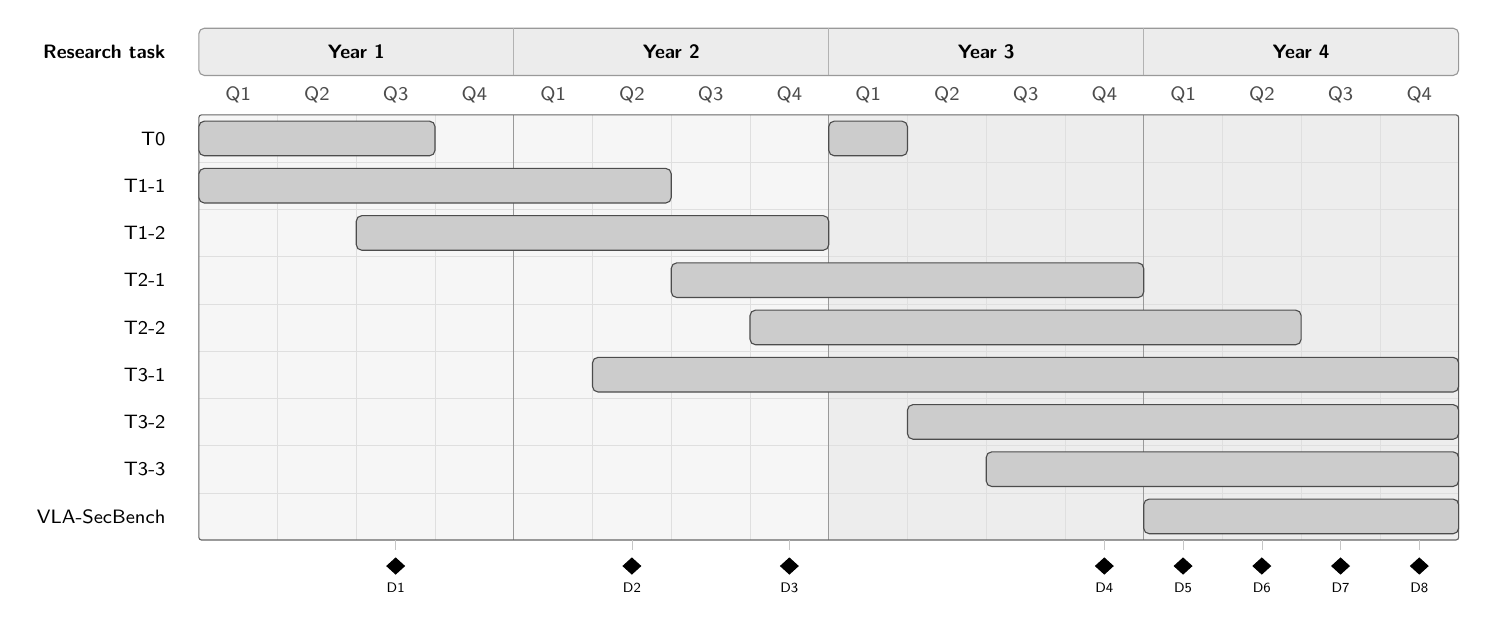
\begin{tikzpicture}[font=\scriptsize\sffamily,
  bar/.style={fill=gray!40, draw=black!70, rounded corners=2pt},
  ]
  %%% activity-band background shading %%%
  \fill[gray!7]  (0,-4.0) rectangle (8,1.4);
  \fill[gray!14] (8,-4.0) rectangle (16,1.4);

  %%% horizontal row separators %%%
  \foreach \hy in {0.80,0.20,-0.40,-1.00,-1.60,-2.20,-2.80,-3.40}
    \draw[very thin, gray!25] (0,\hy) -- (16,\hy);

  %%% vertical quarter gridlines %%%
  \foreach \gx in {1,2,3,5,6,7,9,10,11,13,14,15}
    \draw[very thin, gray!25] (\gx,-4.0) -- (\gx,1.4);
  %%% year boundary lines %%%
  \foreach \gx in {4,8,12}
    \draw[thin, black!40] (\gx,-4.0) -- (\gx,1.4);
  %%% outer chart border %%%
  \draw[black!60, rounded corners=1pt] (0,-4.0) rectangle (16,1.4);

  %%% year header band %%%
  \fill[gray!15, draw=black!40, rounded corners=2pt] (0,1.9) rectangle (16,2.5);
  \foreach \gx in {4,8,12} \draw[black!30] (\gx,1.9) -- (\gx,2.5);
  \node[font=\scriptsize\bfseries\sffamily] at (2,2.2)  {Year 1};
  \node[font=\scriptsize\bfseries\sffamily] at (6,2.2)  {Year 2};
  \node[font=\scriptsize\bfseries\sffamily] at (10,2.2) {Year 3};
  \node[font=\scriptsize\bfseries\sffamily] at (14,2.2) {Year 4};

  %%% quarter tick numbers %%%
  \foreach \g in {1,...,16} {
    \pgfmathtruncatemacro{\qn}{mod(\g-1,4)+1}
    \node[font=\scriptsize\sffamily, text=black!70] at (\g-0.5,1.65) {Q\qn};
  }

  %%% left-hand labels %%%
  \node[anchor=east, font=\scriptsize\bfseries\sffamily] at (-0.3,2.2)  {Research task};
  \node[anchor=east] at (-0.3,1.10)  {T0};
  \node[anchor=east] at (-0.3,0.50)  {T1-1};
  \node[anchor=east] at (-0.3,-0.10) {T1-2};
  \node[anchor=east] at (-0.3,-0.70) {T2-1};
  \node[anchor=east] at (-0.3,-1.30) {T2-2};
  \node[anchor=east] at (-0.3,-1.90) {T3-1};
  \node[anchor=east] at (-0.3,-2.50) {T3-2};
  \node[anchor=east] at (-0.3,-3.10) {T3-3};
  \node[anchor=east] at (-0.3,-3.70) {VLA-SecBench};

  %%% research-task bars (active quarters) %%%
  \fill[bar] (0,0.88)   rectangle (3,1.32);   % T0  Y1Q1-Y1Q3
  \fill[bar] (8,0.88)   rectangle (9,1.32);   % T0  Y3Q1 refresh
  \fill[bar] (0,0.28)   rectangle (6,0.72);   % T1-1 Y1Q1-Y2Q2
  \fill[bar] (2,-0.32)  rectangle (8,0.12);   % T1-2 Y1Q3-Y2Q4
  \fill[bar] (6,-0.92)  rectangle (12,-0.48); % T2-1 Y2Q3-Y3Q4
  \fill[bar] (7,-1.52)  rectangle (14,-1.08); % T2-2 Y2Q4-Y4Q2
  \fill[bar] (5,-2.12)  rectangle (16,-1.68); % T3-1 Y2Q2-Y4Q4
  \fill[bar] (9,-2.72)  rectangle (16,-2.28); % T3-2 Y3Q2-Y4Q4
  \fill[bar] (10,-3.32) rectangle (16,-2.88); % T3-3 Y3Q3-Y4Q4
  \fill[bar] (12,-3.92) rectangle (16,-3.48); % Benchmark Y4Q1-Y4Q4

  %%% deliverable markers along the bottom axis %%%
  \foreach \mx/\ml in {2.5/D1, 5.5/D2, 7.5/D3, 11.5/D4, 12.5/D5, 13.5/D6, 14.5/D7, 15.5/D8} {
    \draw[very thin, gray!45] (\mx,-4.0) -- (\mx,-4.13);
    \fill[black, draw=black] (\mx,-4.23) -- (\mx-0.11,-4.33) -- (\mx,-4.43) -- (\mx+0.11,-4.33) -- cycle;
    \node[font=\tiny\sffamily, anchor=north, inner sep=1pt] at (\mx,-4.5) {\ml};
  }
\end{tikzpicture}%
}\vspace{-2ex}
\caption{Work-plan timeline with anticipated project start on (May~2027): Year~1 (May~2027--Apr~2028) to Year~4 (May~2030--Apr~2031). Quarters marked as Q1--Q4 and deliverables as D1--D8. {\textbf{Deliverables:} \textbf{D1} model and data repository with reproducible baselines (Y1Q3); \textbf{D2} ABBP with evasion and poisoning variants (Y2Q2); \textbf{D3} STAP and TTDA with open-source attack release (Y2Q4); \textbf{D4} TACD and AGAT with open-source defense release (Y3Q4); \textbf{D5} cross-model, cross-embodiment transferability matrix (Y4Q1); \textbf{D6} safety benchmark across models, embodiments, and tasks (Y4Q2); \textbf{D7} multimodal attack and defense evaluation (Y4Q3); \textbf{D8} VLA-SecBench v1.0 and the action-interpretability toolkit publicly released (Y4Q4).}}
\label{fig:workplan_timeline}
\end{figure*}